

\documentclass[11pt]{article}
\usepackage[utf8]{inputenc}
\usepackage{geometry}
\usepackage{graphicx}
\usepackage{hyperref}
\usepackage{amsmath}
\usepackage{listings}
\usepackage{xcolor}
\usepackage{float}
\usepackage{subcaption}
\usepackage{algorithm}
\usepackage{algpseudocode}
\usepackage{booktabs} % For prettier tables
\usepackage{siunitx}
\usepackage{amssymb}
\usepackage{url}

% Set page margins
\geometry{a4paper, margin=1in}

% Set up code listing style
\lstset{
    basicstyle=\ttfamily,
    commentstyle=\color{gray},
    keywordstyle=\color{blue},
    stringstyle=\color{red},
    showstringspaces=false,
    captionpos=b
}

\title{Automated Lung CT Segmentation -  DICOM to UNet Analysis: Medical Imaging Coursework Report}
\author{Vishal Jain}
\date{\today}

\begin{document}

\maketitle

\tableofcontents
Word count: 2132 words (including appendix)
\newpage

\section{Introduction}
This report presents the work done for the Medical Imaging coursework. The aim of the coursework was to explore part of the LCTSC Lung CT dataset and build a 2D image segmentation model using the UNet architecture. This report will provide an overview of the steps taken, the results obtained and present a critical discussion of the results.

\section{Module 1: Handling DICOM data}
The code and the data for the analysis described in this section can be found in the \texttt{\url{src/explore_dicoms.ipynb}} notebook and the \texttt{Dataset} directory, respectively.

\subsection{Dataset Exploration}
To investigate the dicoms, the \texttt{pydicom} library was used to read the DICOM files from the different cases. The first tag that was investigated was the \texttt{PatientIdentityRemoved} tag. This tag is used to indicate whether the patient identity has been removed from the DICOM file. The tag was checked for all the cases and it was found that the value was \texttt{YES} for all cases. However, investigating the meta data revealed a few cases still had sensitive information. This was removed by the script \texttt{src/de\_identify\_dataset.py} which is called during the set up instructions shown on the README.md file. The next set of tags investigated were the tags that are relevant to the stratification of the data. These tags were the \texttt{PatientSex}, \texttt{KVP}, \texttt{Manufacturer}, and \texttt{ModelName}. The summary of this information is presented in Table \ref{tab:patient_meta}. Note, patient age would also have been included however it was not available for any of the cases in the dataset.

\begin{table}[h]
    \centering
    \begin{tabular}{|l|c|c|l|l|}
    \hline
    \textbf{Case ID} & \textbf{Sex} & \textbf{KVP} & \textbf{Model Name} & \textbf{Manufacturer} \\ \hline
    000 & M & 120 & Sensation Open & SIEMENS \\ \hline
    001 & M & 120 & Sensation Open & SIEMENS \\ \hline
    002 & M & 120 & Sensation Open & SIEMENS \\ \hline
    003 & F & 120 & Sensation Open & SIEMENS \\ \hline
    004 & F & 120 & Sensation Open & SIEMENS \\ \hline
    005 & M & 120 & Sensation Open & SIEMENS \\ \hline
    006 & M & 120 & Sensation Open & SIEMENS \\ \hline
    007 & M & 120 & Sensation Open & SIEMENS \\ \hline
    008 & F & 120 & Sensation Open & SIEMENS \\ \hline
    009 & F & 120 & Biograph 40 & SIEMENS \\ \hline
    010 & F & 120 & Sensation Open & SIEMENS \\ \hline
    011 & F & 120 & Sensation Open & SIEMENS \\ \hline
    \end{tabular}
    \caption{Summary of patient data}
    \label{tab:patient_meta}
\end{table}

When training a model, it's crucial to ensure that both train and test sets are similarly stratified to avoid introducing bias. In this dataset, all fields except sex are consistent across cases. Consequently, only patient sex has been used for stratification. Given the even distribution between male and female cases, no resampling techniques were required to enforce balance.

The subsequent analysis focused on voxel-related metadata. These fields were checked to ensure consistency across cases. The fields examined included voxel size, slice thickness, image orientation, rescale intercept, rescale slope, patient position, and pixel array shape. It was found that all fields were consistent across all cases except in the rescale intercept values, in which case 9 had a value of -1000 compared to the rest of the cases -1024. To investigate that the distribution of intensities is consistent across cases. The intensity histograms were plot for all cases, which are shown in Figure \ref{fig:intensity_histograms}. It is important to note that the voxel intensities were winsorised to the 1st and 99th percentiles to remove outliers before plotting the histograms.

\begin{figure}[H]
    \centering
    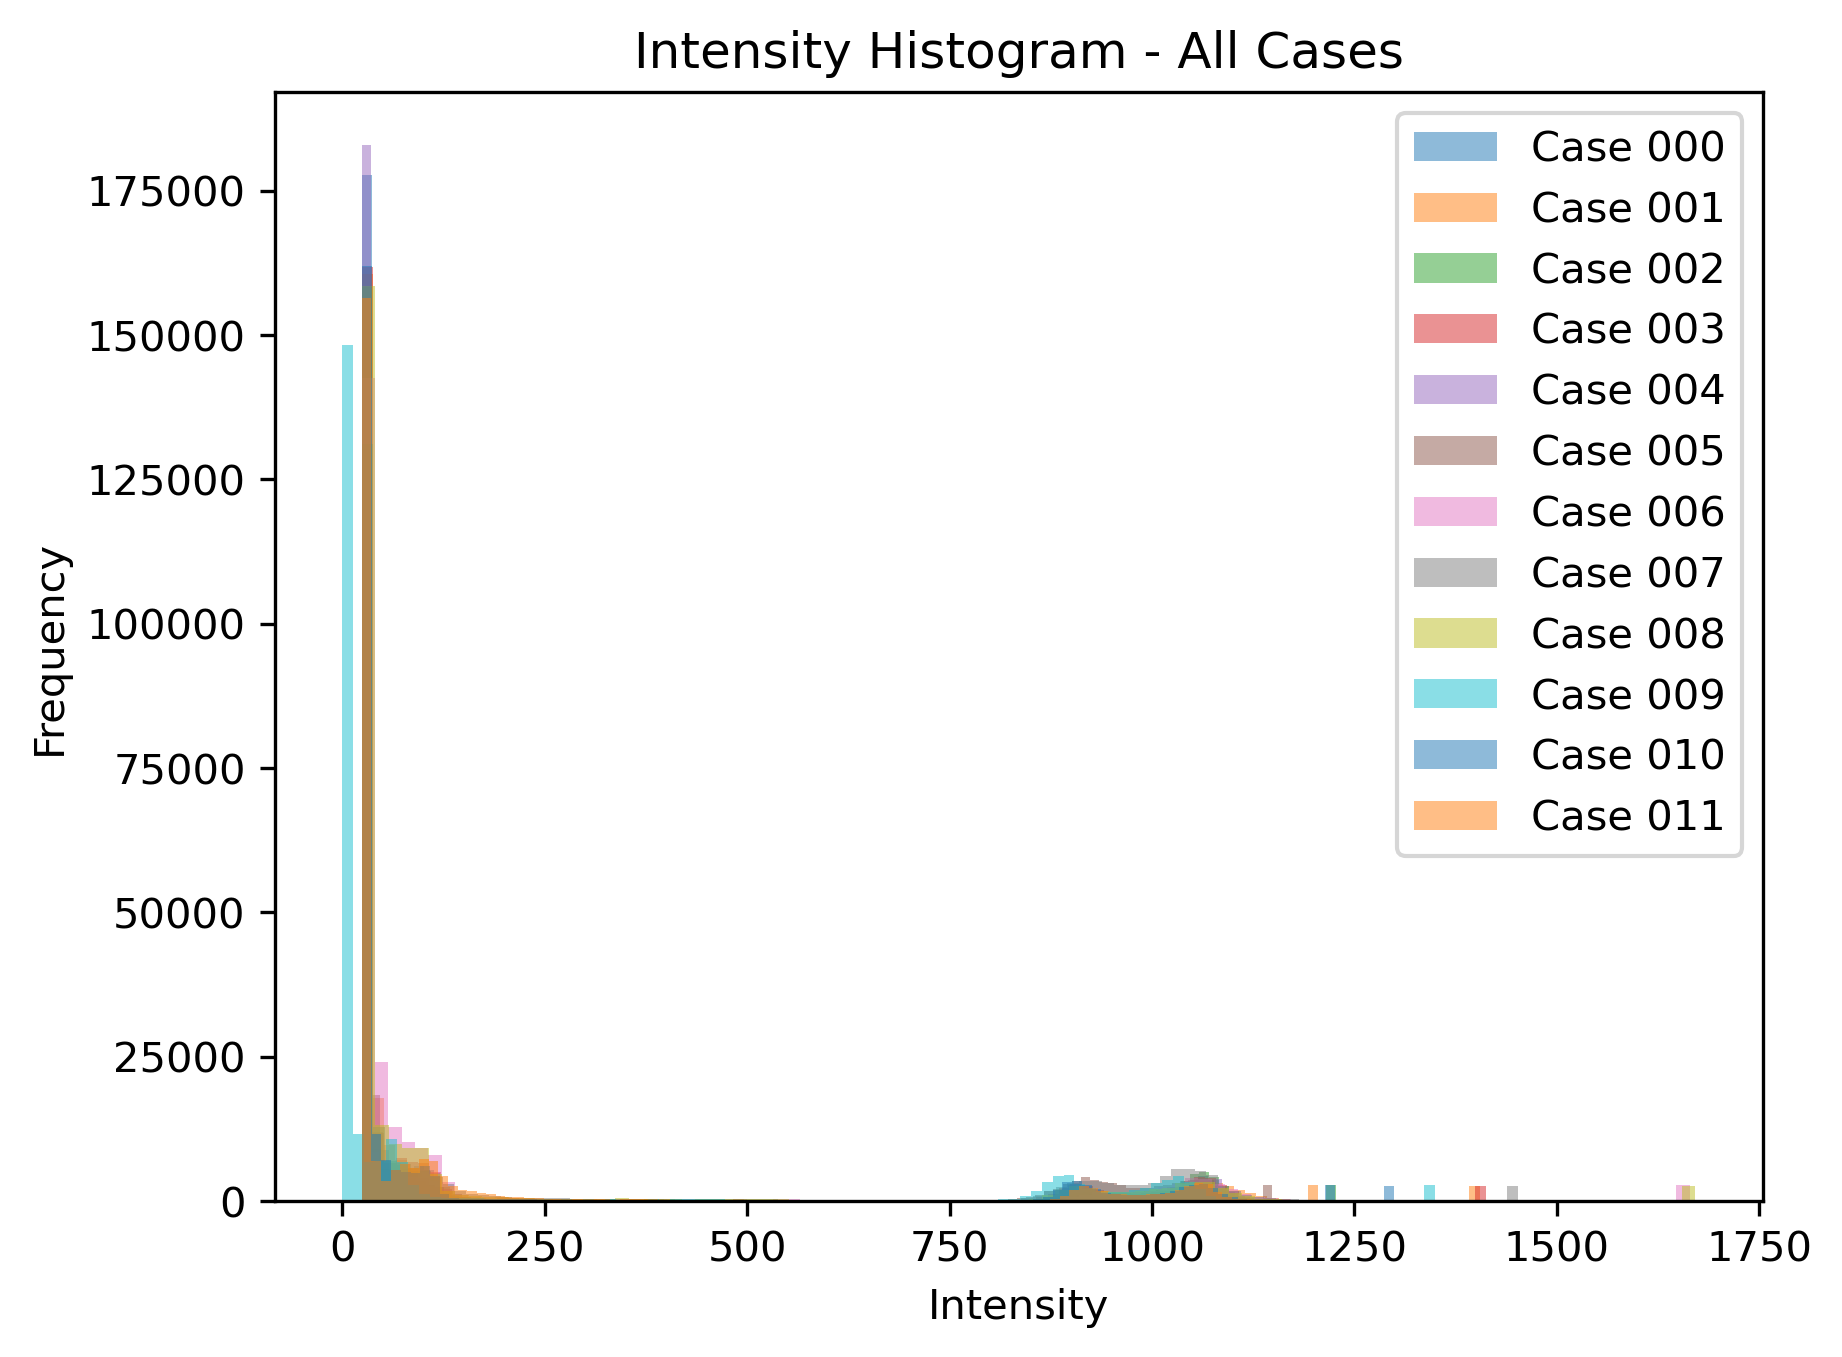
\includegraphics[width=0.8\textwidth]{figs/intensity_histogram_orig.png}
    \caption{Intensity histograms for all cases}
    \label{fig:intensity_histograms}
\end{figure}

These histograms demonstrate that the intensity distributions are consistent across the different cases in dataset. However, case 9 is identifiable by a histogram peak slightly shifted to the left relative to the peaks of other cases, illustrating a minor deviation in its intensity distribution. To correct for this, all the cases intensities were transformed to the Hounsfield unit scale using the rescale intercept and rescale slope values. The new intensity histograms are shown in Figure \ref{fig:hounsfield_histograms_hu}. The histograms are now consistent across all cases, indicating that the intensities are now on the same scale. Note, a deliberate choice was made not to window these intensities and centre them around the mean intensity of the lungs. This is because the model may learn useful features from contrast within the other tissues that would be lost if the intensities were windowed.

\begin{figure}[H]
    \centering
    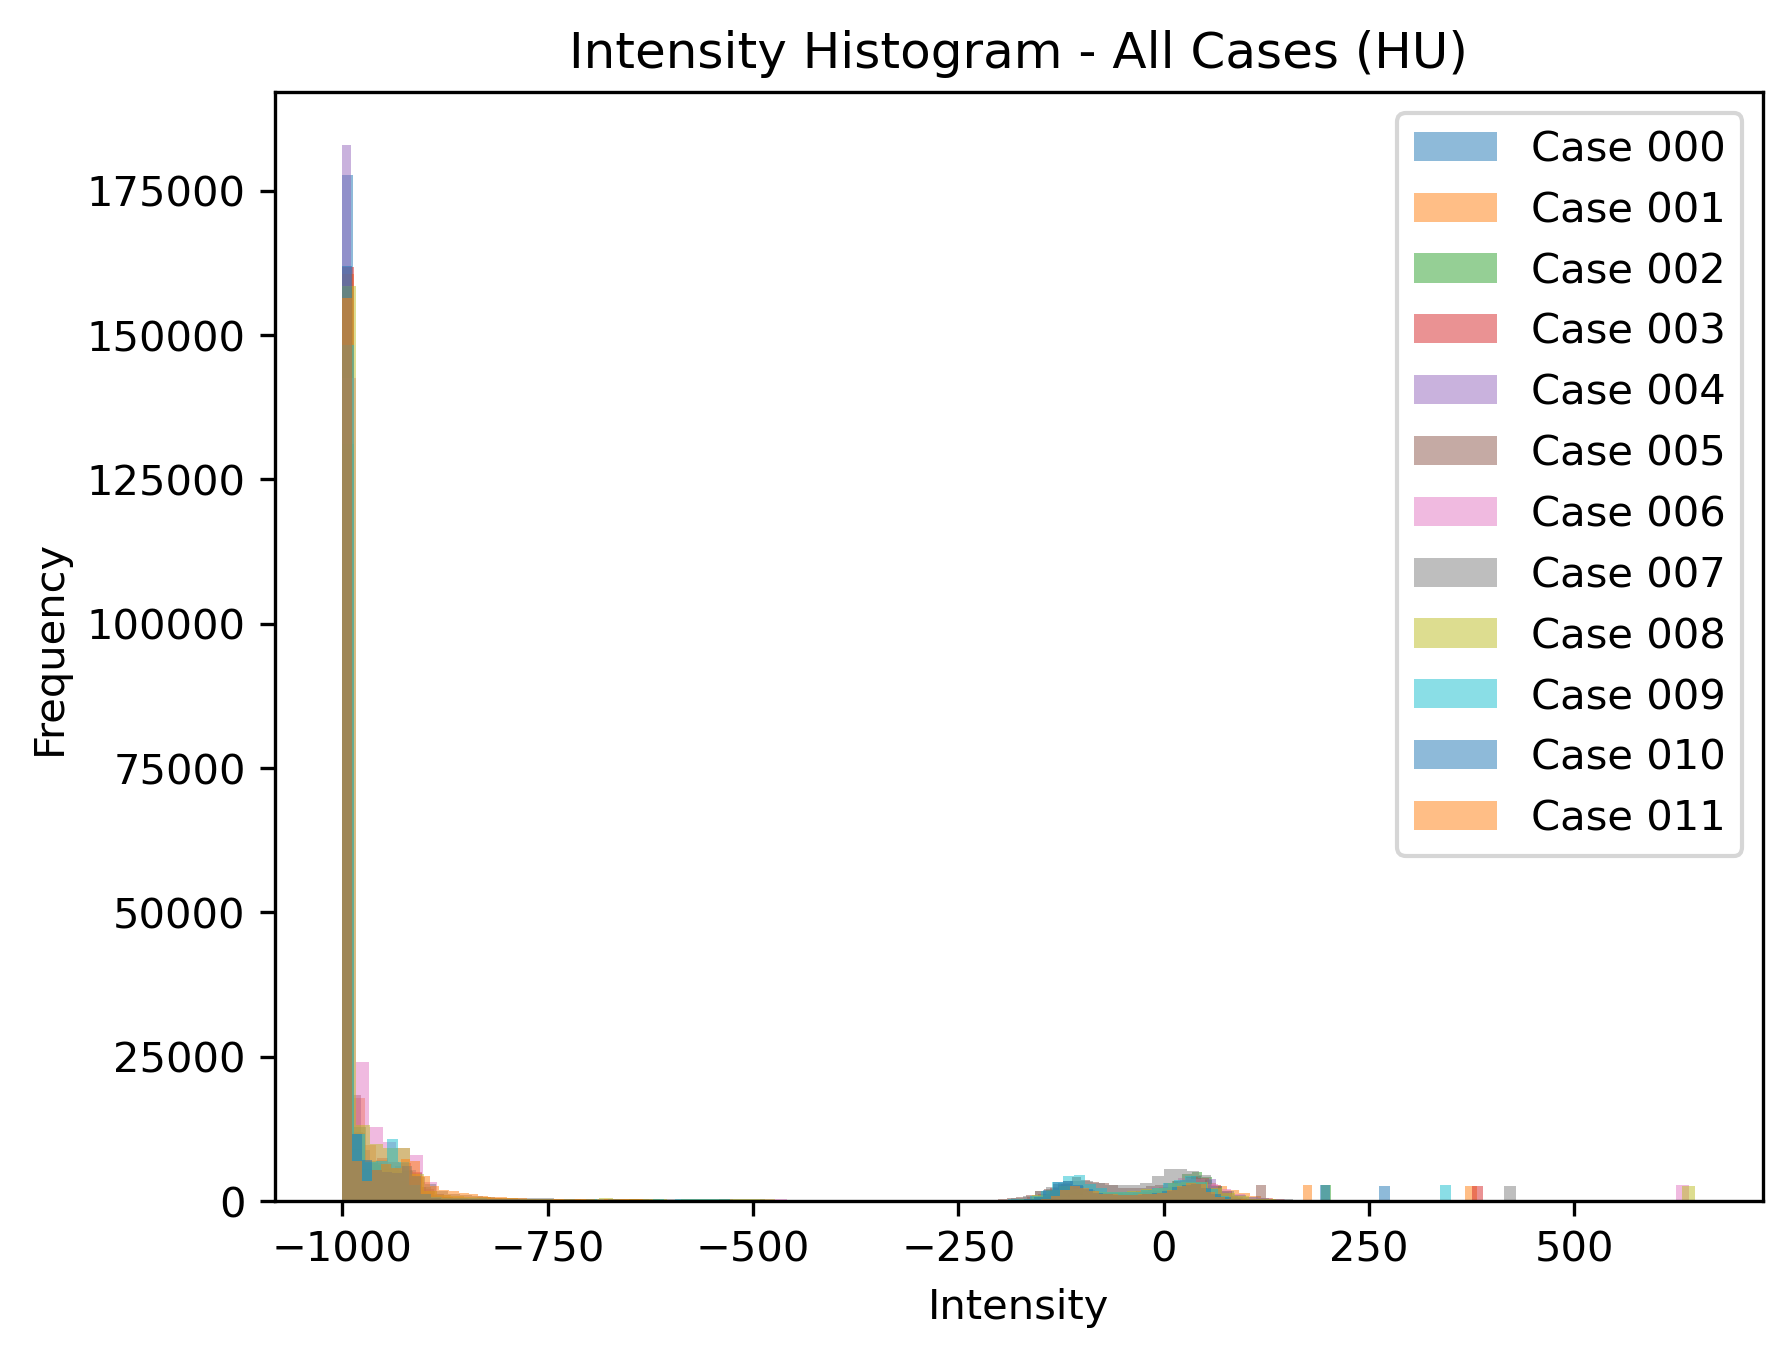
\includegraphics[width=0.8\textwidth]{figs/intensity_histogram_hu.png}
    \caption{Hounsfield unit histograms for all cases}
    \label{fig:hounsfield_histograms_hu}
\end{figure}

\subsection{Converting DICOMs to 3D Numpy Arrays}
The next step was to convert the DICOM files to 3D numpy arrays. The relevant code for this can be found in the \texttt{\url{src/utils.py}} script under the functions \texttt{\url{load\_npz}} and \texttt{\url{dicom\_dir\_to\_3D\_arr}}. To load the dicoms related to a single case into a 3D array the following steps were taken:

\begin{enumerate}
    \item Read all the DICOM files in the directory using \texttt{pydicom.dcmread}.
    \item Sort the files by their $z$ coordinate using the third element of the \texttt{ImagePositionPatient} attribute.
    \item For each DICOM file, extract the pixel array using the \texttt{pixel\_array} attribute. Then, convert the pixel values to Hounsfield Units (HU) by applying the formula $HU = pixel\_value \times RescaleSlope + RescaleIntercept$. The values for these coefficients are taken from the DICOM file's metadata.
    \item Use the \texttt{numpy.stack} function to stack the 2D pixel arrays, now converted to Hounsfield Units, sorted by their $z$ coordinate along a new axis. This operation creates a 3D numpy array, where each 2D slice corresponds to a single DICOM image, arranged in the correct order along the patient's $z$ axis.
\end{enumerate}

To load the masks which were provided in the form of a \texttt{.npz} file, 
\texttt{numpy.load} function was used to load the file and extract the mask array.
To verify proper alignment between the 3D image and mask arrays, they were reviewed in ITKSNAP, a standard medical image viewer. Due to ITKSNAP's format limitations, the .npz mask files could not be loaded natively and were first converted to NIfTI. Creating a NIfTI file from a numpy array necessitates specifying an affine matrix—a 4x4 matrix mapping voxel to world coordinates. Rather than deriving this matrix from DICOM metadata, both the DICOM images (which are natively viewable in ITKSNAP) and masks were converted to NIfTI using an identity affine matrix, simplifying the process. The code for which can be found in the \texttt{\url{src/utils.py}} script under the function \texttt{\url{make_niftis}}. The image and lung mask volumes were then reviewed for each case in ITKSNAP and were confirmed found to be correctly aligned by the loading process defined previosly. An example of the image and mask for case 000 is shown in Figure \ref{fig:itksnap}. It is worth noting that because the affine matrix was not derived from DICOM metadata, the images and masks were not displayed in their correct physical dimensions in ITKSNAP. However, this does not affect the segmentation process as the model is trained on the 3D numpy arrays directly, all that matters is the shape and alignment of the image and mask arrays.

\begin{figure}[H]
    \centering
    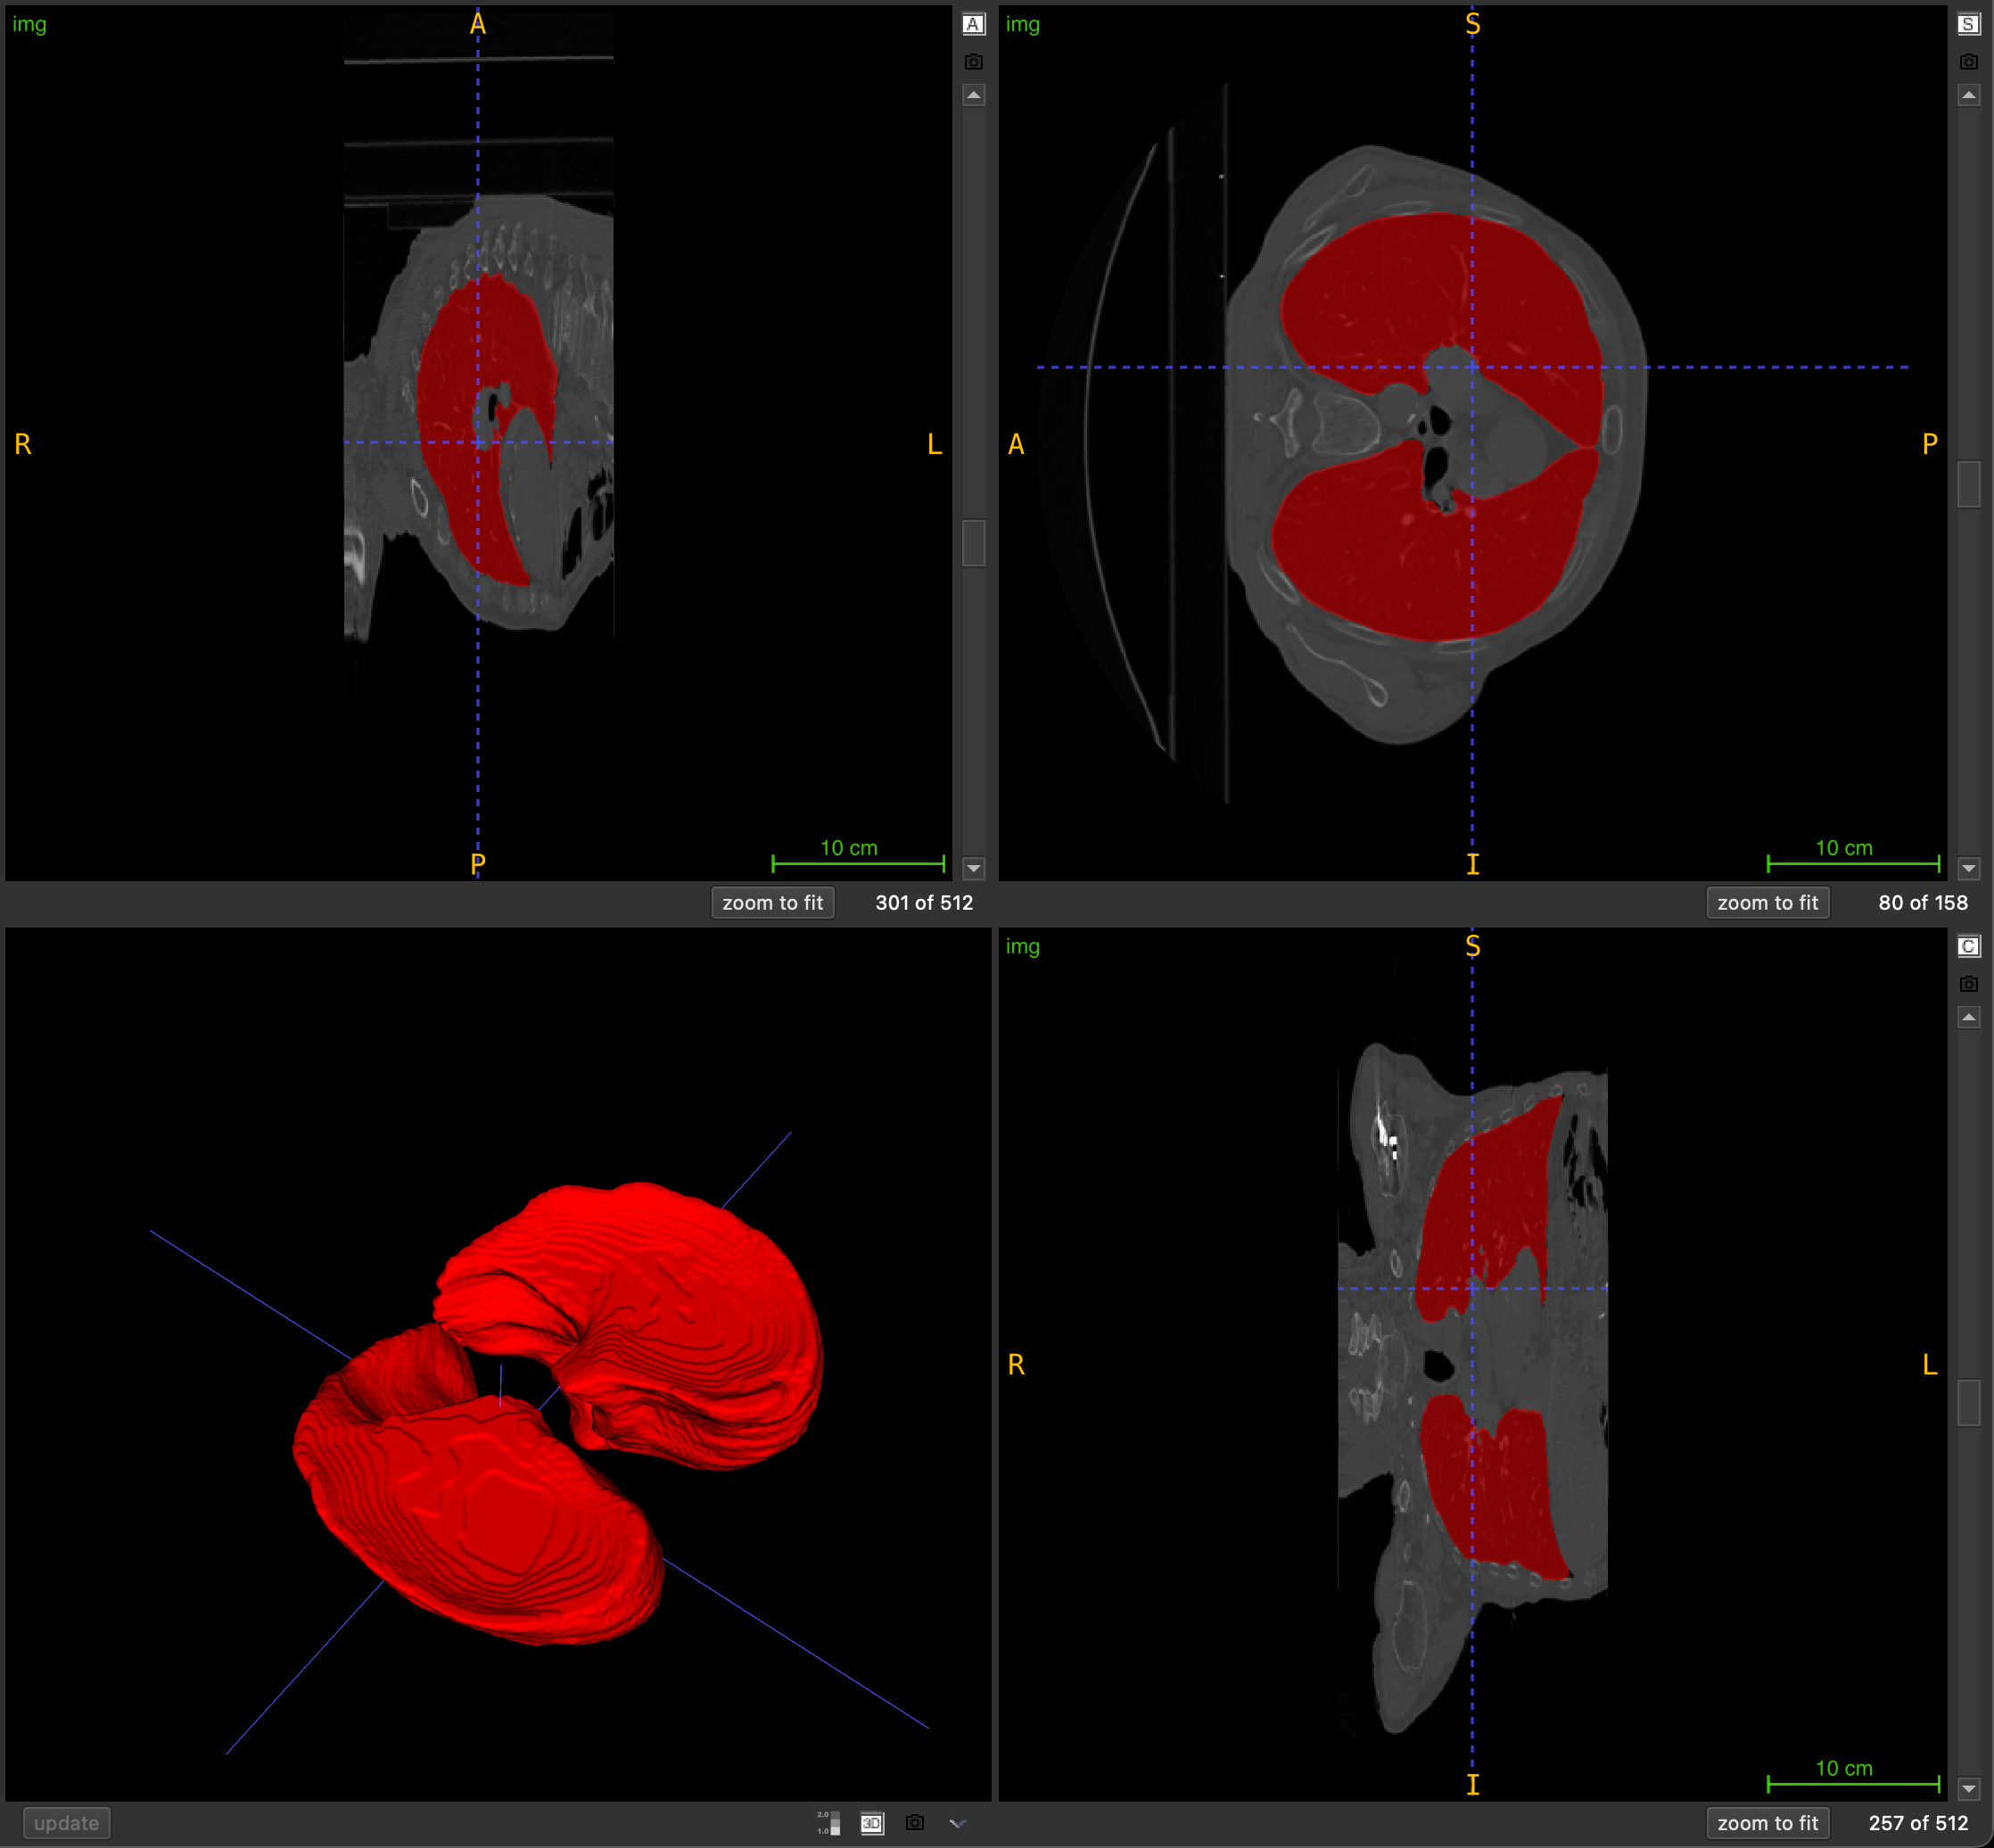
\includegraphics[width=0.8\textwidth]{figs/itksnap.png}
    \caption{ITKSNAP view of the image and mask for case 001}
    \label{fig:itksnap}
\end{figure}


\section{Module 2: UNet-based segmentation}
This section describes the training and evaluation of a 2D UNet model for lung segmentation. The code for this analysis can be found in the \texttt{\url{src/train.py}} and \texttt{\url{src/test.py}} scripts. 

\subsection{Model Architecture}
% Describe model architecture
The model architecture utilises a 2D UNet, comprising an encoder and a decoder. The encoder features a sequence of double convolutional layers, each separated by max pooling layers. A double convolutional layer consists of two consecutive blocks, with each block performing the operations of convolution, batch normalisation, and ReLU activation in sequence. Following this, downsampling is achieved through max pooling, complemented by a dropout layer for regularisation. Conversely, the decoder is structured around a series of upconvolutional layers, each succeeded by a double convolutional layer. During the decoding process, feature maps from the encoder are concatenated with the upsampled feature maps. The model architecture is shown in Figure \ref{fig:unet}.
\begin{figure}[H]
    \centering
    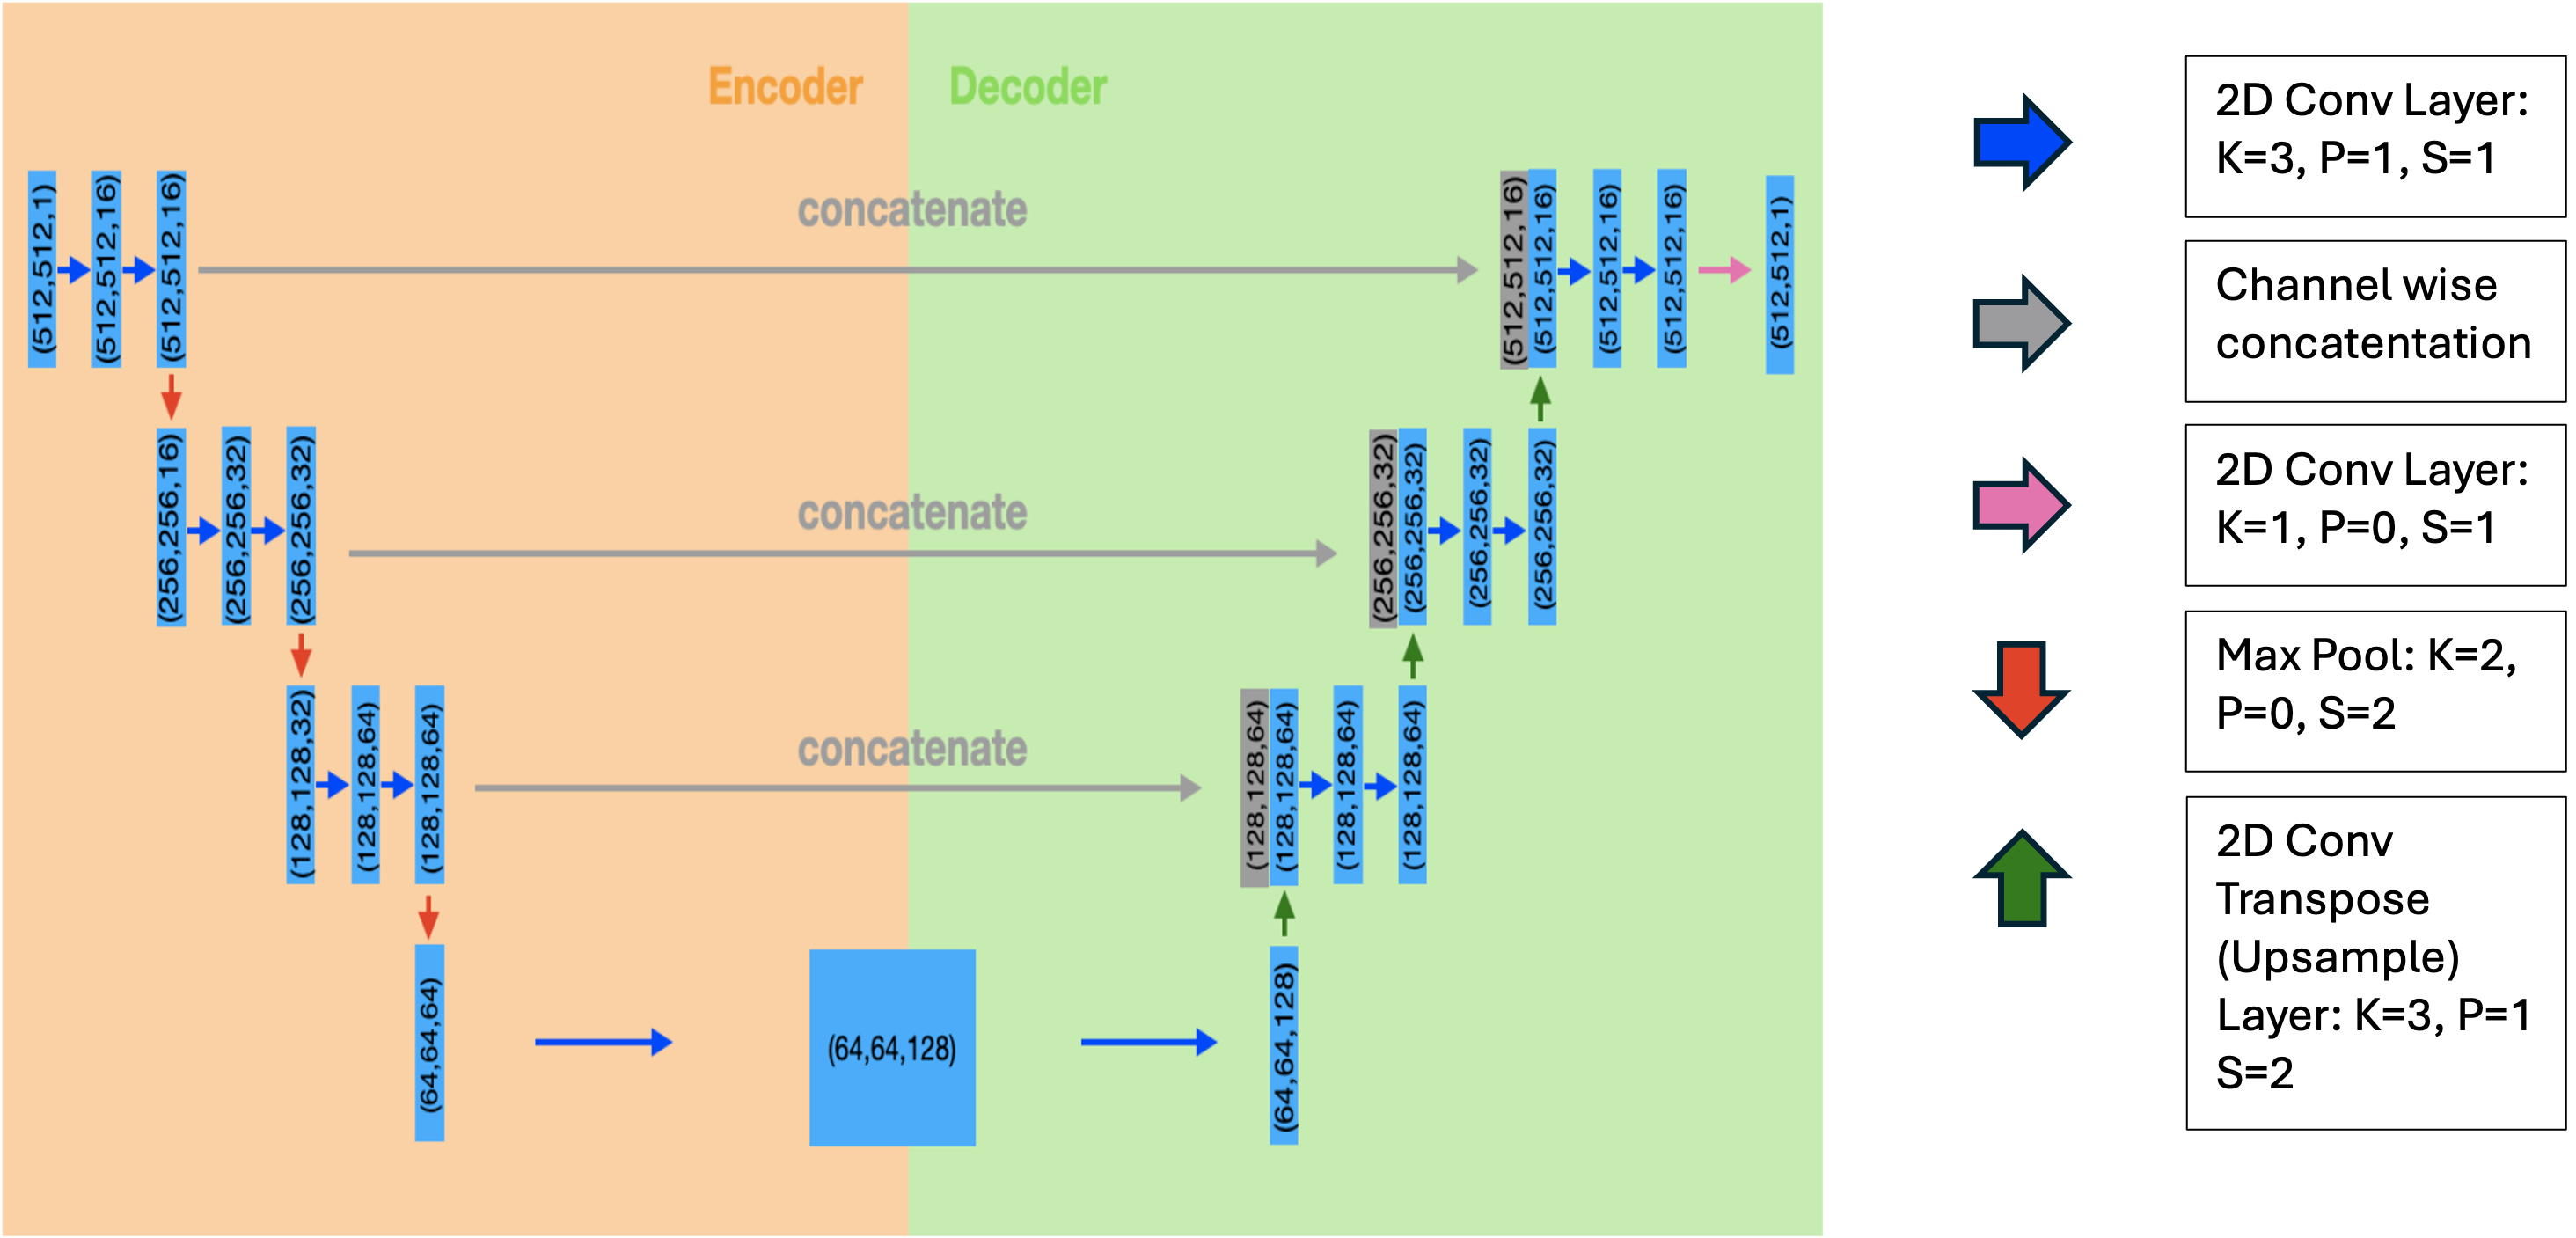
\includegraphics[width=0.8\textwidth]{figs/unet.png}
    \caption{Diagram of the UNet architecture used, illustrating the dimensions of the input at each layer in the format HxWxC, where H is height, W is width, and C represents the number of channels. The accompanying legend (right) employs the following key: K for kernel size, S for stride, and P for padding.}
    \label{fig:unet}
\end{figure}

\subsection{Data Splits and Preprocessing}
The dataset is divided into training and testing sets using a 2:1 ratio. To avoid data leakage, all slices from a specific patient are allocated to the same set, ensuring the model isn't trained and tested on slices from the same case. Additionally, cases are distributed between the splits to maintain a 50-50 male-female ratio, respecting the dataset's diversity and preventing the model from developing biases towards features associated with a single gender.
Finally, the data is winsorised and normalised to the range [0,1]. This process was applied to each slice independently.  

\subsection{Training}
% Training the model - loss function, optimizer, learning rate, epochs, batch size.
The model was trained for 10 epochs, using a batch size of 3 and the adam optimiser with a learning rate of 0.1.
The loss function used was the binary cross entropy loss via the \texttt{BCEWithLogitsLoss} class from the PyTorch library in combination with a custom implementation of soft dice loss. The custom implementation can be found in the \texttt{\url{src/losses.py}} script. The soft dice loss is a metric that measures the overlap between the predicted and ground truth masks. It is particularly relevant for imbalanced datasets, as is the case here where the lung region is significantly smaller than the background. Both loss terms are equally weighted in the final loss function. The average loss and binary accuracy for each epoch are plotted in Figure \ref{fig:loss_plot}. Note how the binary accuracy is already 95\% after the first epoch and only shows a rough increase  of 4\% over the next 9 epochs. Compared with the loss which has a more consistent decrease over the 10 epochs, changing by about 30\% in total. This shows how the soft dice loss is a more sensitive metric than the binary accuracy, which is expected given the imbalanced nature of the dataset.

\begin{figure}[H]
    \centering
    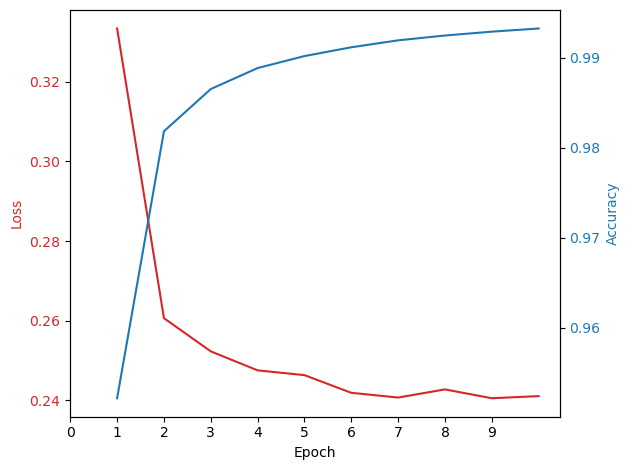
\includegraphics[width=0.8\textwidth]{figs/train_metrics.png}
    \caption{Plot of the average loss and binary accuracy for each epoch during training. The blue line represents the loss, while the red line denotes the binary accuracy.}
    \label{fig:loss_plot}
\end{figure}
\subsection{Evaluation}
To evaluate the model the distribution of dice scores between the train and test set are visualised as histograms in \ref{fig:dice_dist_hist} and boxplots in \ref{fig:dice_dist_box}. The same can be done for the distribution of the binary accuracies. The distributions between the train and test are shown in histogram form in Figure \ref{fig:accuracy_dist_hist} and boxplot form in Figure \ref{fig:accuracy_dist_box}. The summary statistics are presented in table \ref{tab:accuracy_summary}.
The model performance can also be visually assessed by comparing the predicted masks with the ground truth masks for cases with the highest, lowest and typical dice scores (typical here means dice scores that fall in the IQR). This is done in figs \ref{fig:best_train_mask_comparison}, \ref{fig:typical_train_mask_comparison}, \ref{fig:worst_train_mask_comparison} for the train set and in figs \ref{fig:best_test_mask_comparison}, \ref{fig:typical_test_mask_comparison}, \ref{fig:worst_test_mask_comparison} for the test set.

\begin{table}[H]
    \centering
    \begin{tabular}{lcc}
    \hline
    \textbf{Dice Score}          & \textbf{Train Set} & \textbf{Test Set} \\ \hline
    Mean         & 0.943          & 0.949         \\
    Max           & 0.993           & 0.995          \\
    Min          & 0.114           & 0.0877          \\
    Upper Quartile           & 0.986           & 0.990          \\
    Lower Quartile           & 0.965           & 0.977          \\
    Interquartile Range (IQR) & 0.0210           & 0.0129          \\
    Standard Deviation       & 0.118           & 0.117          \\ \hline
    \end{tabular}
    \caption{Train and Test Split Dice Scores}

    \label{tab:dice_scores}
\end{table}
    
\begin{table}[ht]
    \centering
    \begin{tabular}{lcc}
    \toprule
    \textbf{Accuracy}                 & \textbf{Train Set} & \textbf{Test Set}   \\
    \midrule
    Mean       & 0.996      & 0.997      \\
    Max         & 0.999      & 0.998      \\
    Min        & 0.992      & 0.997      \\
    Upper Quartile       & 0.996      & 0.997      \\
    Lower Quartile       & 0.996      & 0.997      \\
    IQR                  & 0.00014    & 0.00023    \\
    Standard Deviation   & 0.00031    & 0.00015    \\
    \bottomrule
    \end{tabular}
    \caption{Train and Test Split Binary Accuracies}

    \label{tab:accuracy_summary}
    \end{table}
    
\begin{figure}[H]
    \centering
    \begin{subfigure}[t]{0.8\textwidth}
        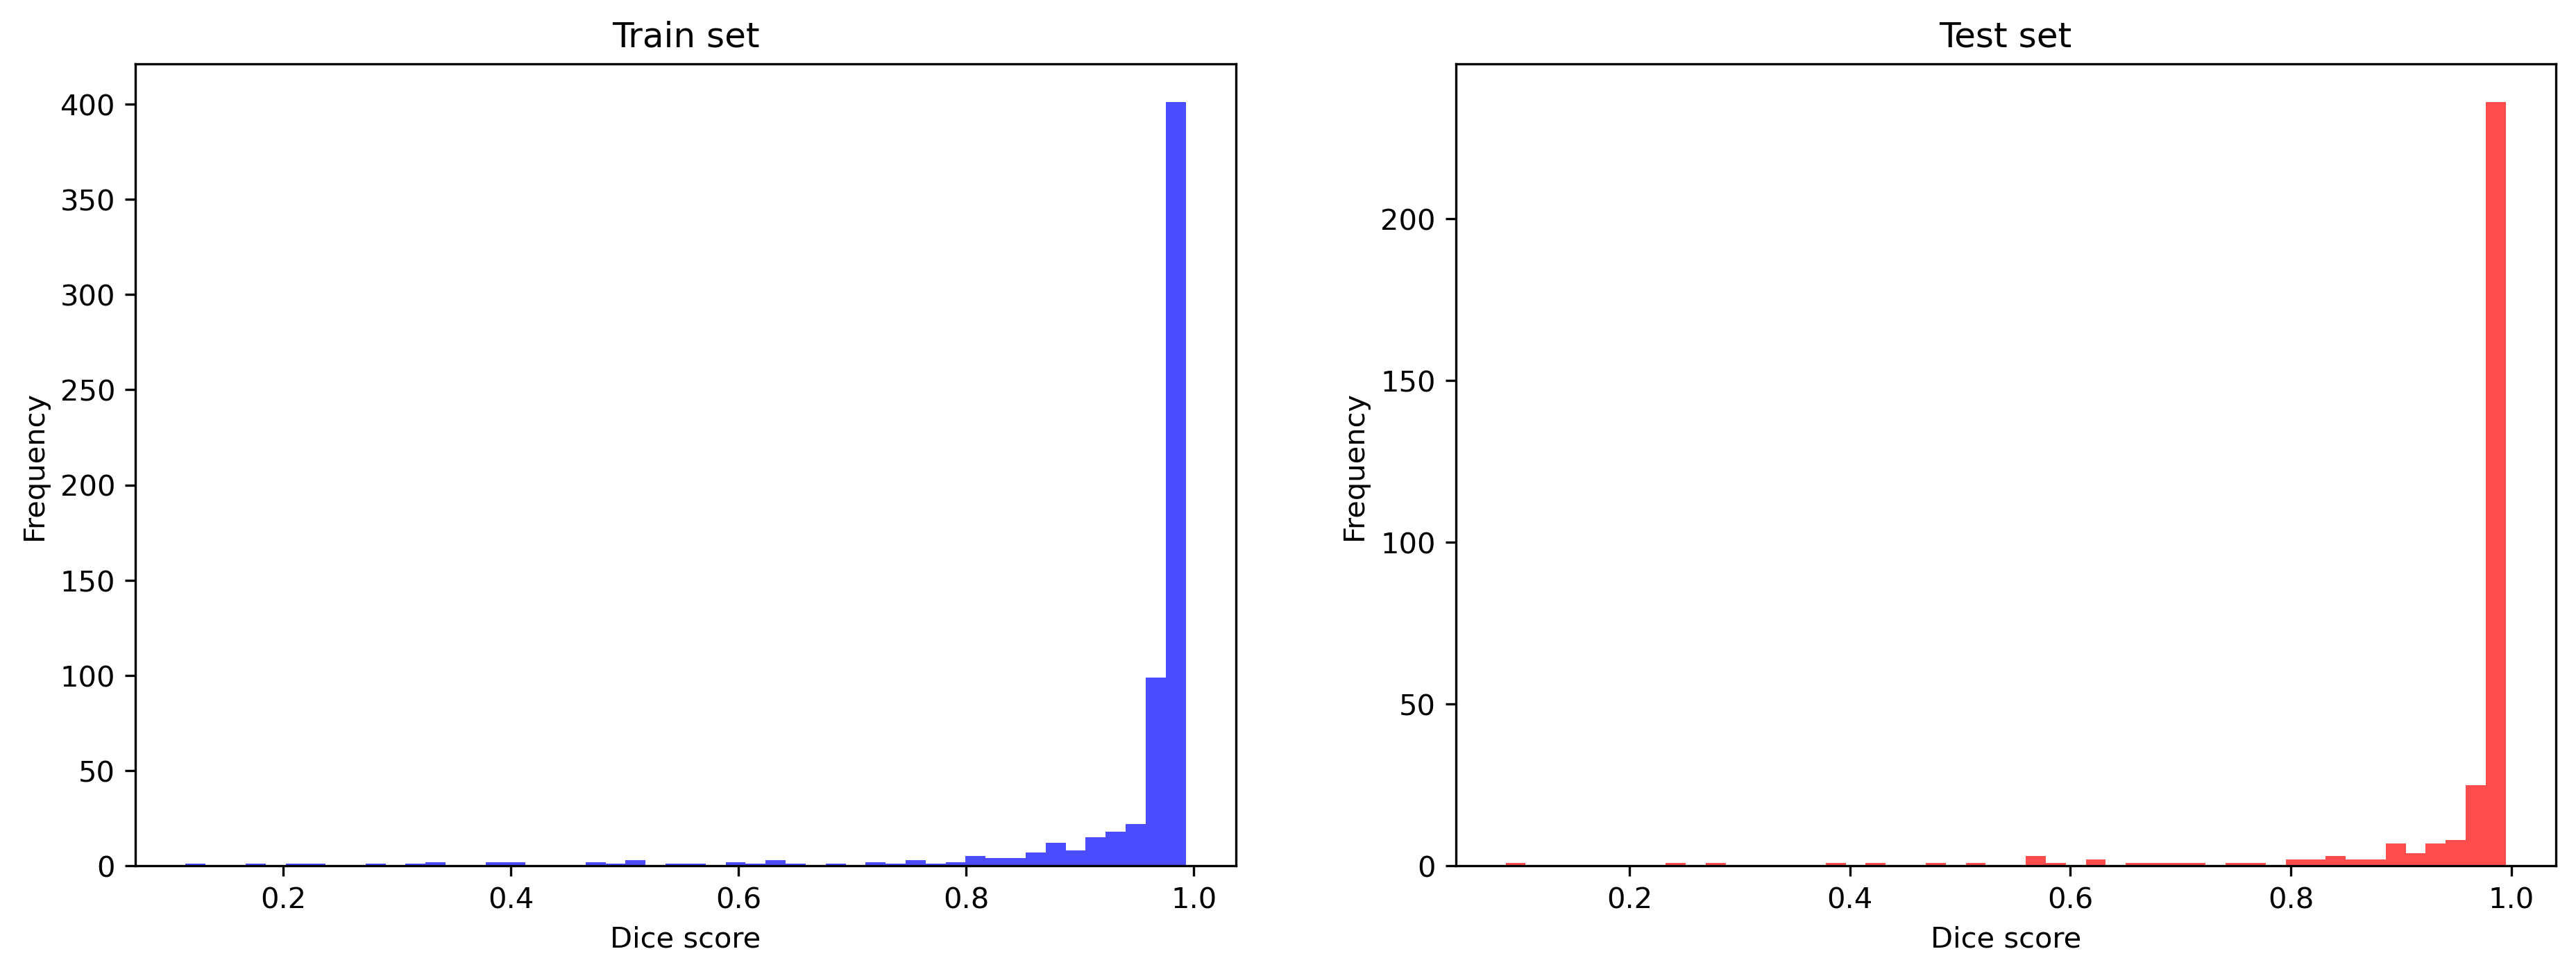
\includegraphics[width=\textwidth]{figs/dice_score_histograms.png}
        \caption{Histogram of dice scores for the train and test sets.}
        \label{fig:normal_dice_dist_hist}
    \end{subfigure}
    \hfill
    \begin{subfigure}[t]{0.8\textwidth}
        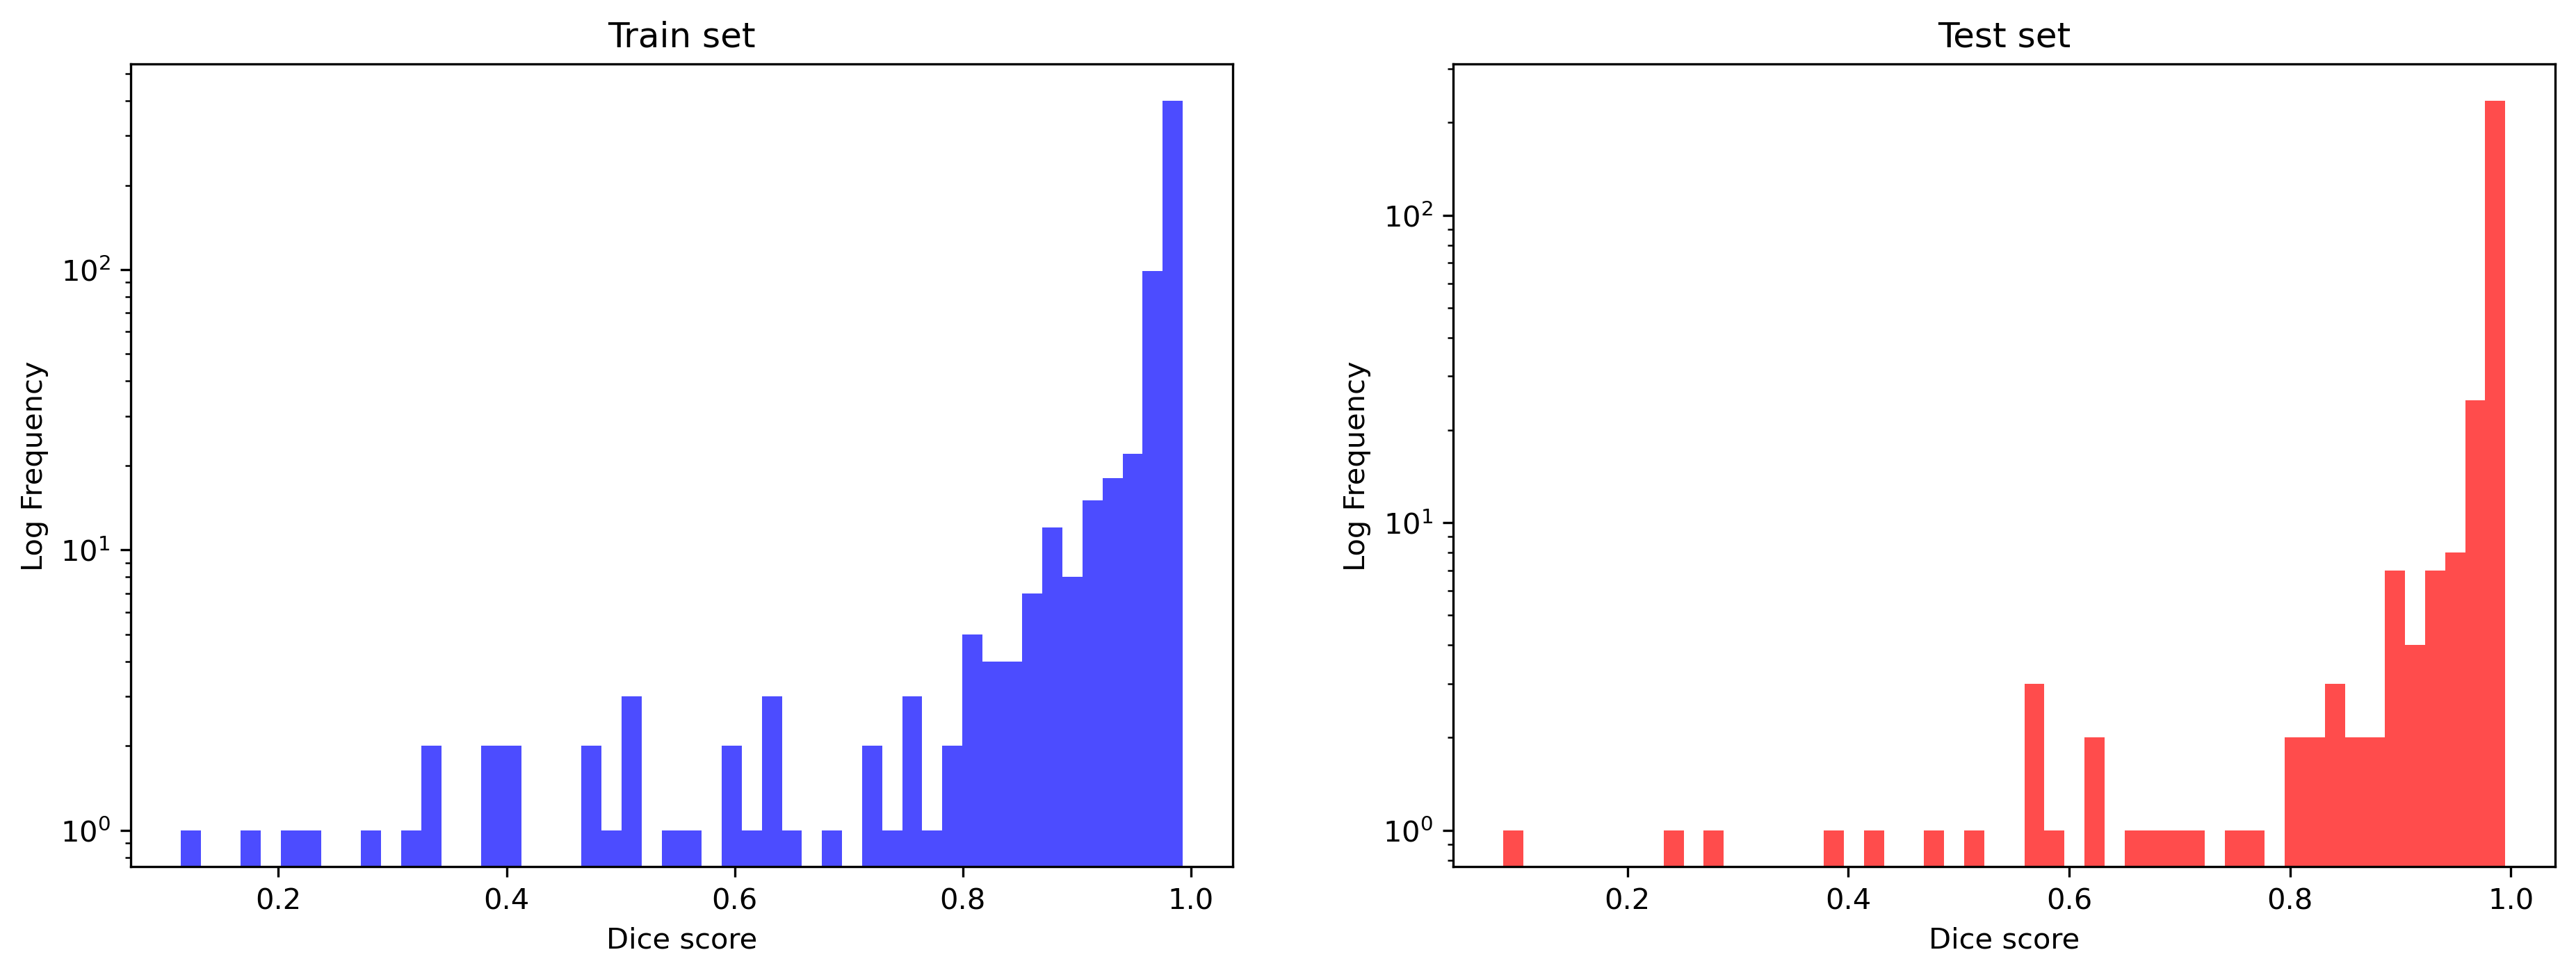
\includegraphics[width=\textwidth]{figs/log_dice_score_histograms.png}
        \caption{Histogram of dice scores for the train and test sets using a log scale for the y-axis.}
        \label{fig:log_dice_dist_hist}
    \end{subfigure}
    \caption{Comparison of dice score distributions for the train and test sets with different y-axis scales.}
    \label{fig:dice_dist_hist}
\end{figure}
\begin{figure}[H]
    \centering
    \begin{subfigure}[t]{0.8\textwidth}
        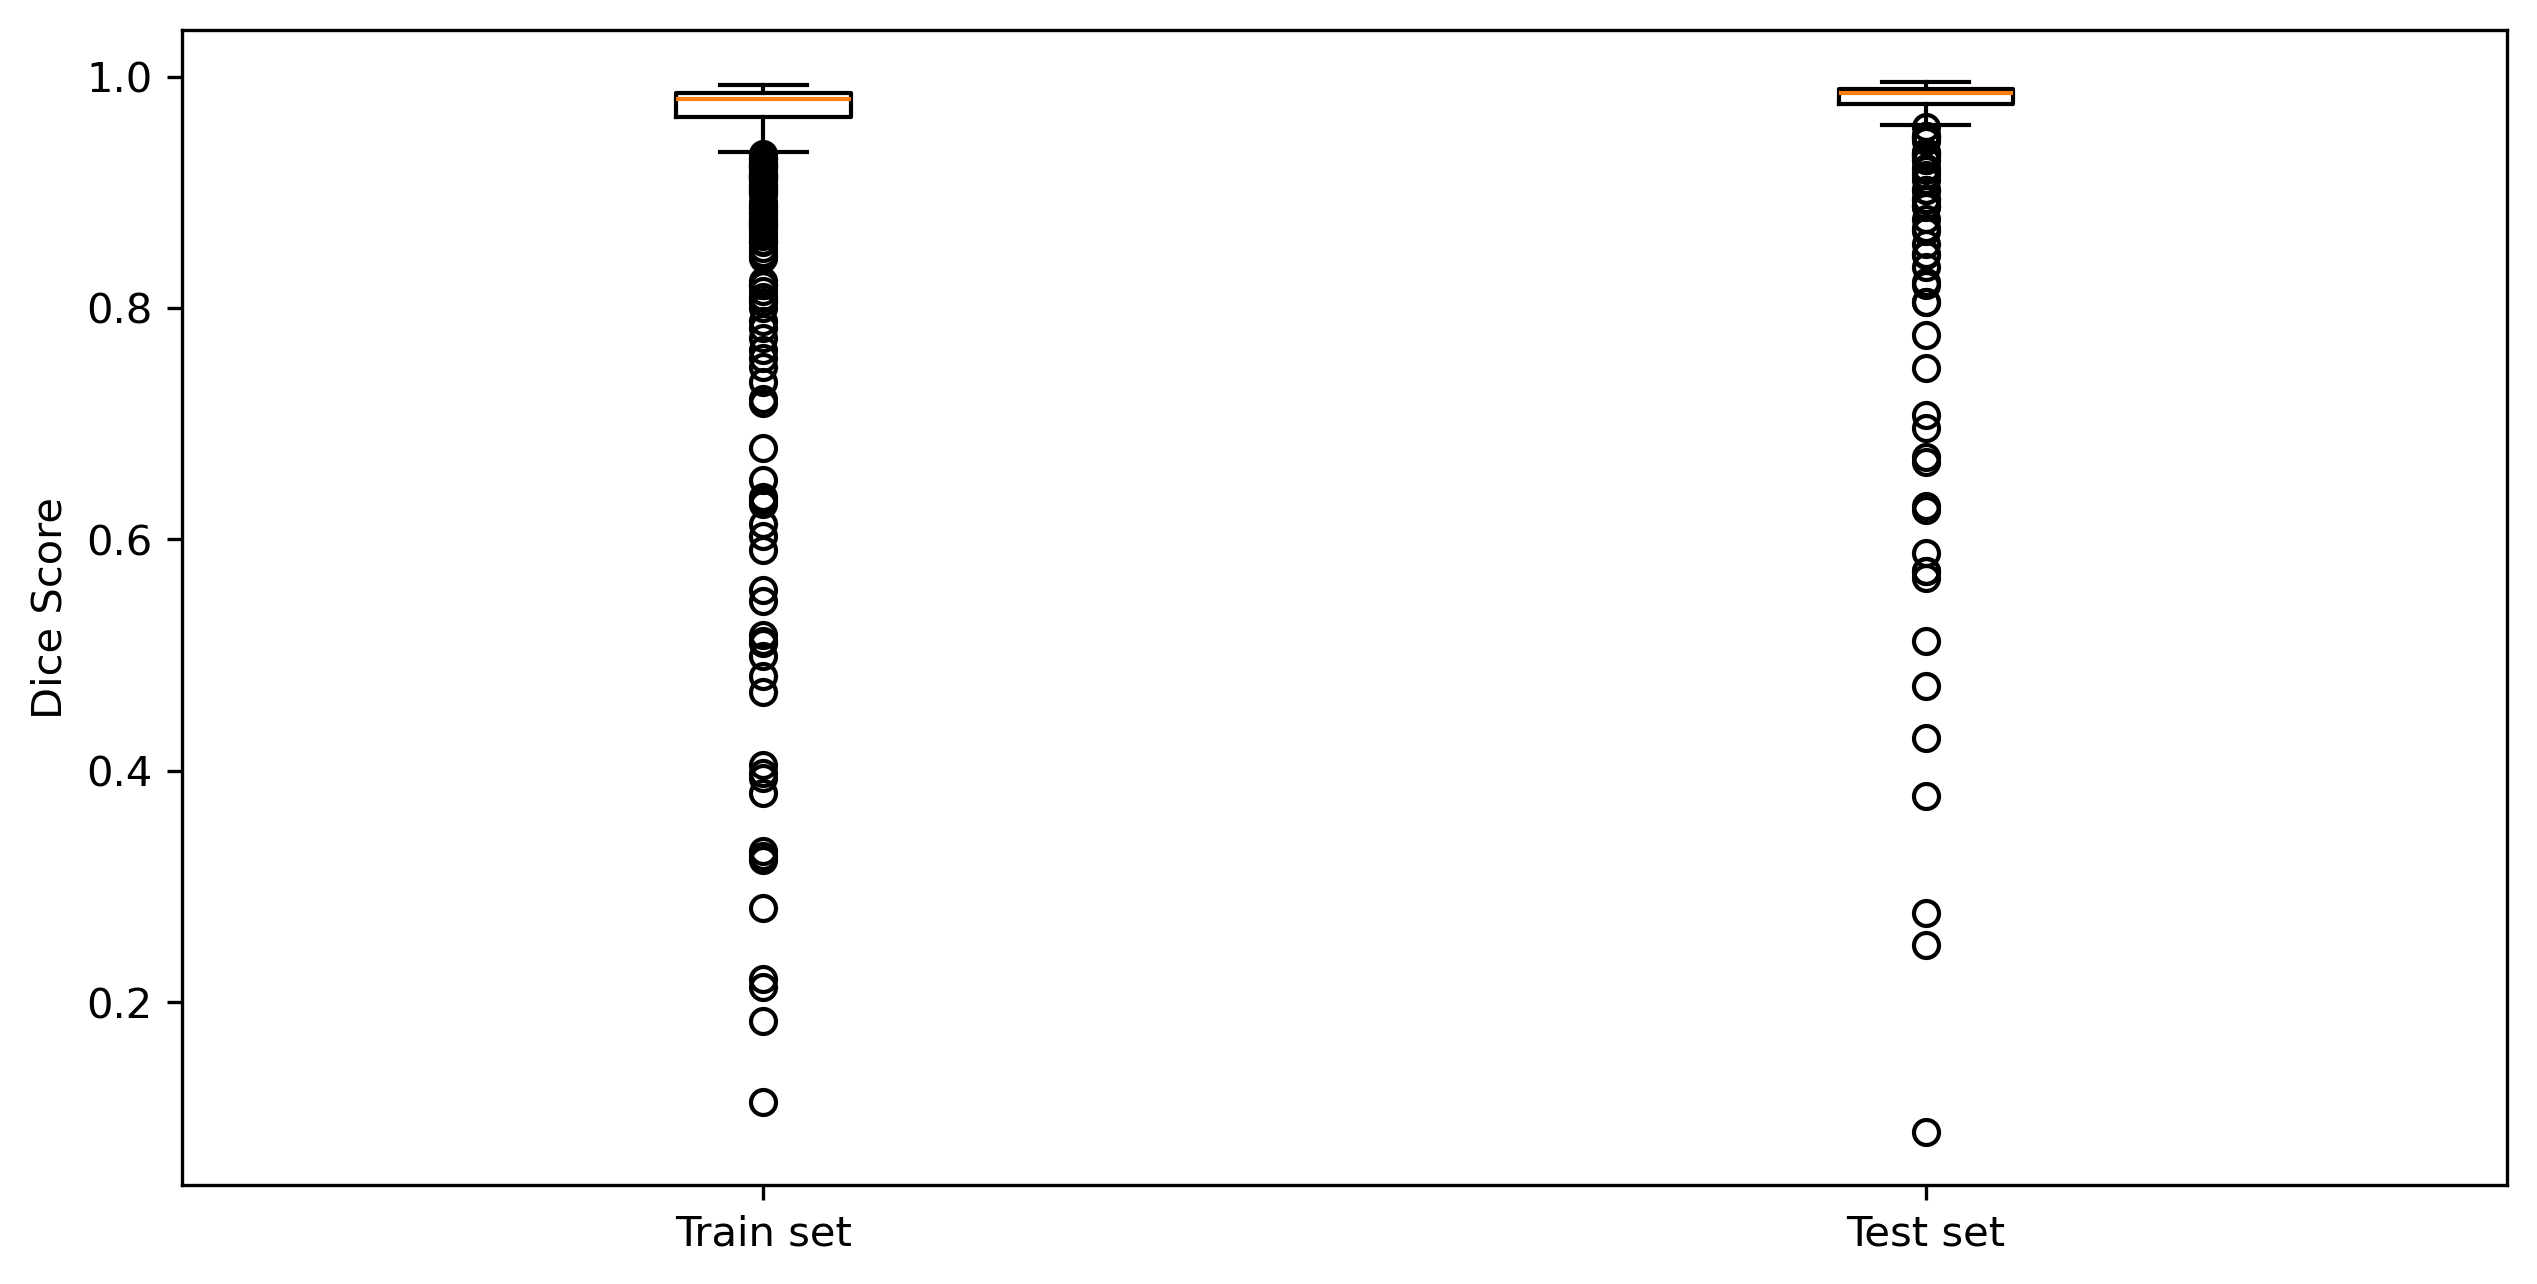
\includegraphics[width=\textwidth]{figs/dice_score_boxplot.png}
        \caption{Boxplot of dice scores for the train and test sets.}
        \label{fig:dice_dist_box_orig}
    \end{subfigure}
    \hfill
    \begin{subfigure}[t]{0.8\textwidth}
        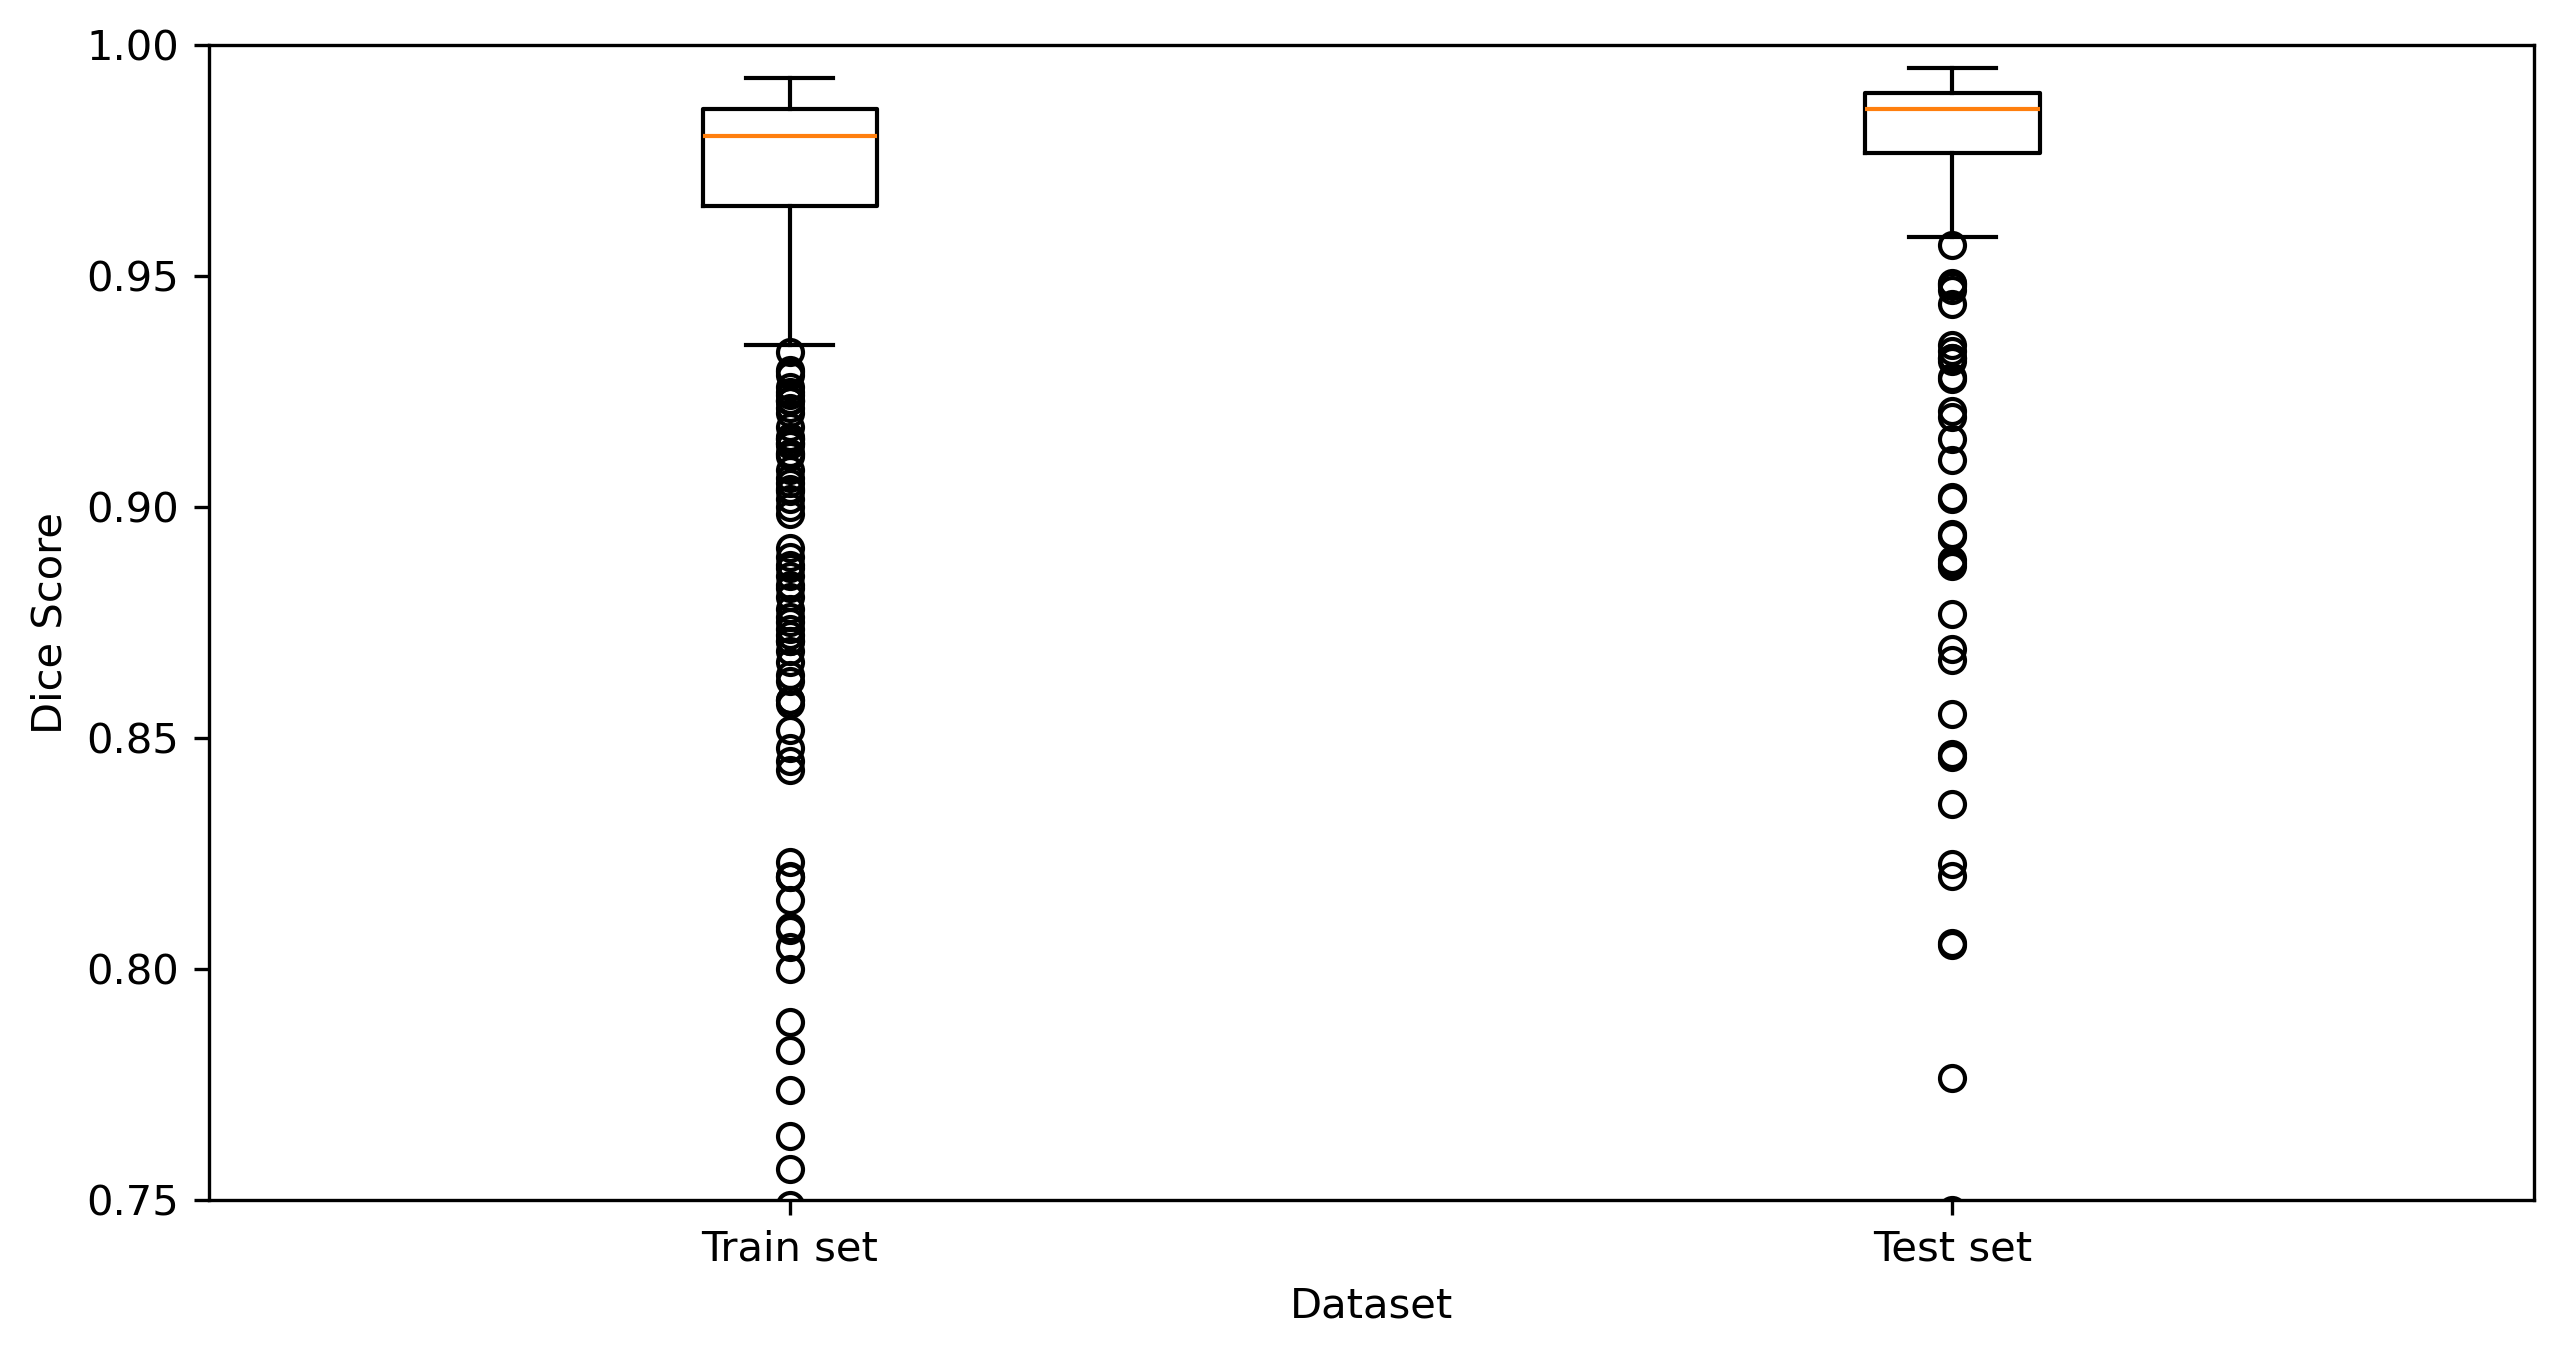
\includegraphics[width=\textwidth]{figs/zoomed_dice_score_boxplot.png}
        \caption{Zoomed in.}
        \label{fig:dice_dist_box_zoomed}
    \end{subfigure}
    \caption{Comparison of the dice score distributions between the train and test splits using box plots. Top: original box plot, bottom: zoomed in box plot.}
    \label{fig:dice_dist_box}
\end{figure}

\begin{figure}[H]
    \centering
    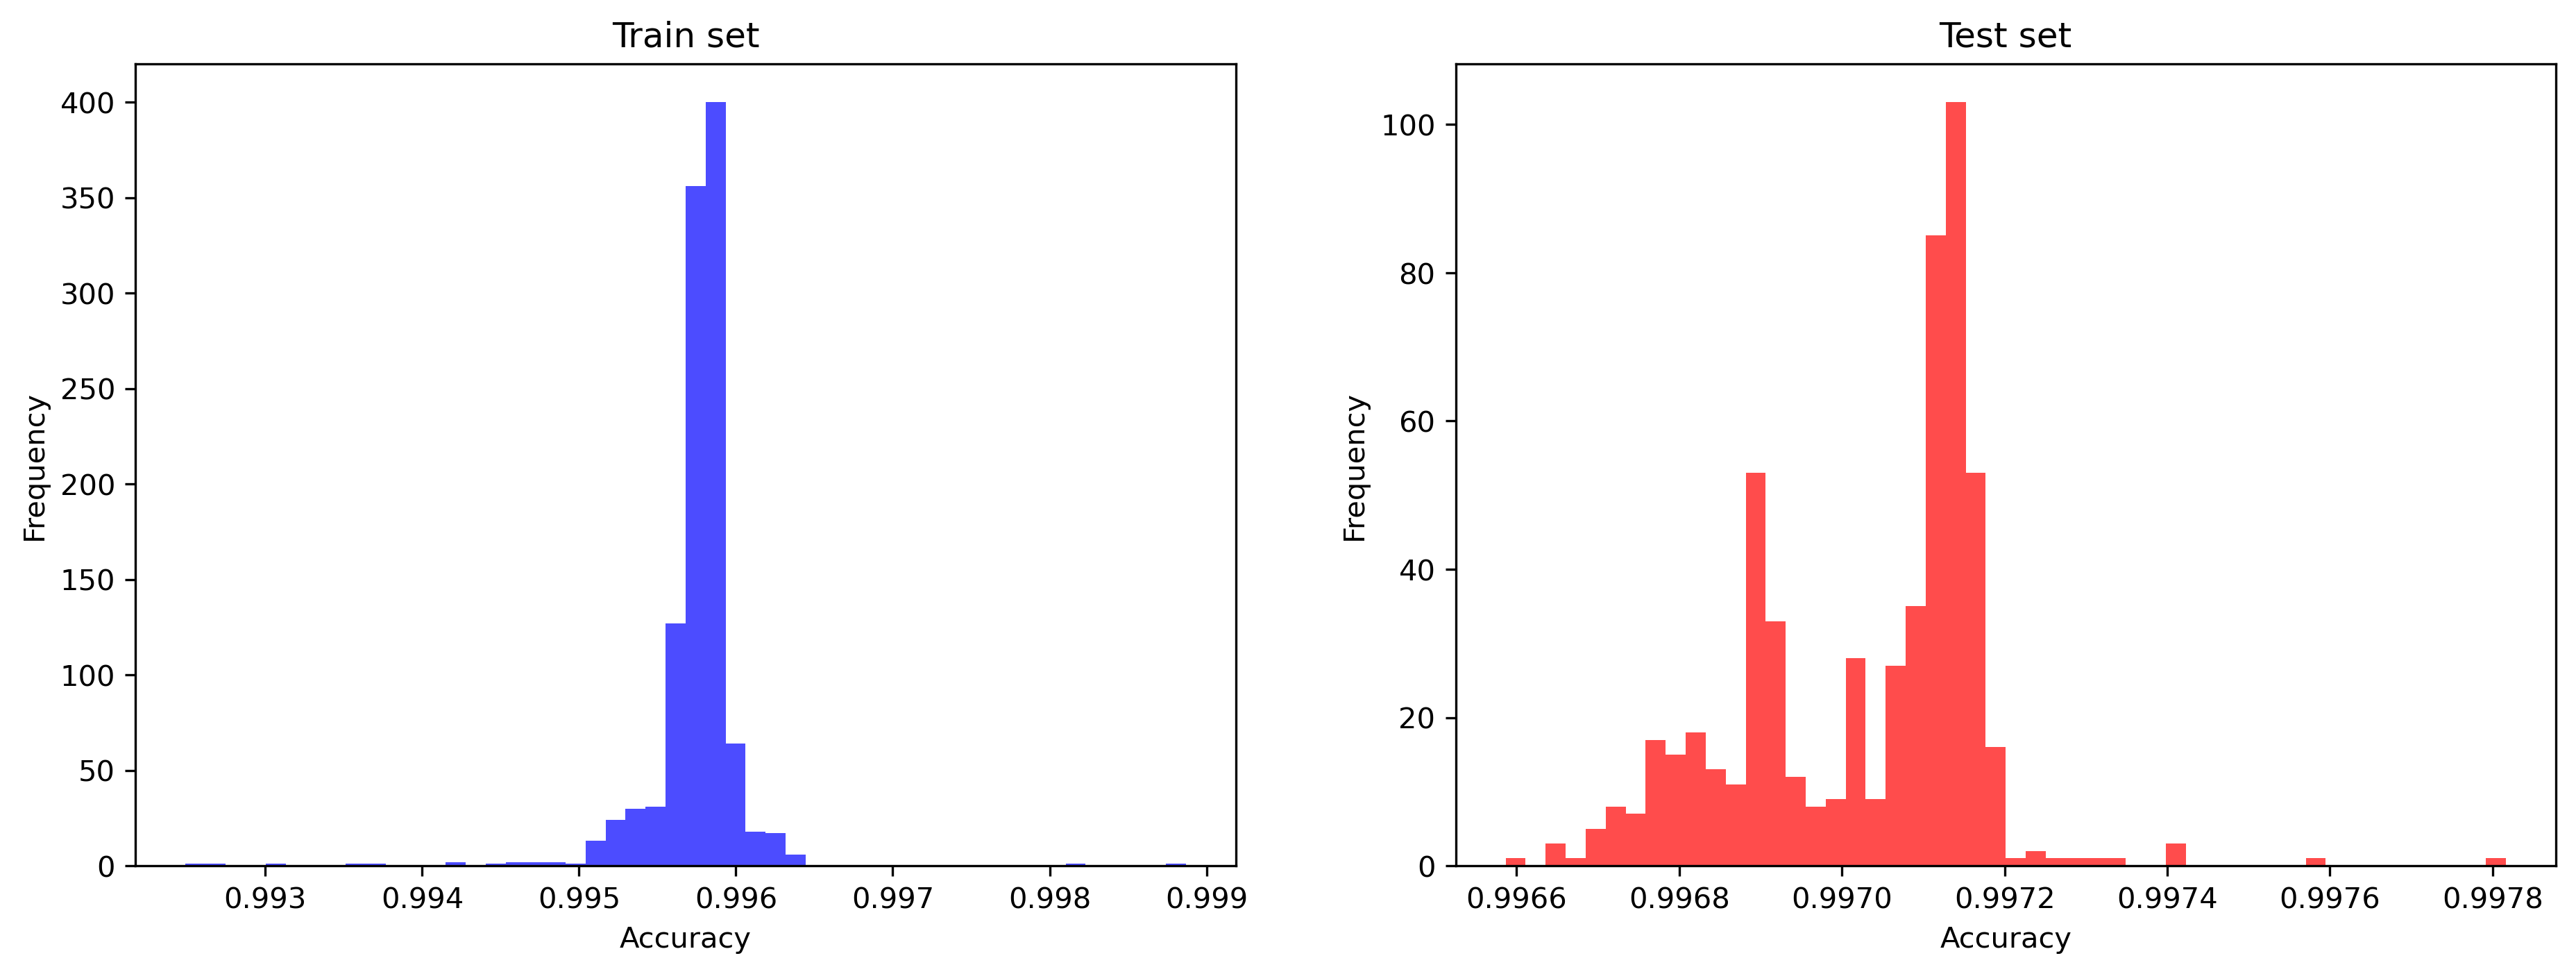
\includegraphics[width=0.8\textwidth]{figs/accuracy_histograms.png}
    \caption{Histogram of binary accuracies for the train and test sets.}
    \label{fig:accuracy_dist_hist}
\end{figure}

\begin{figure}[H]
    \centering
    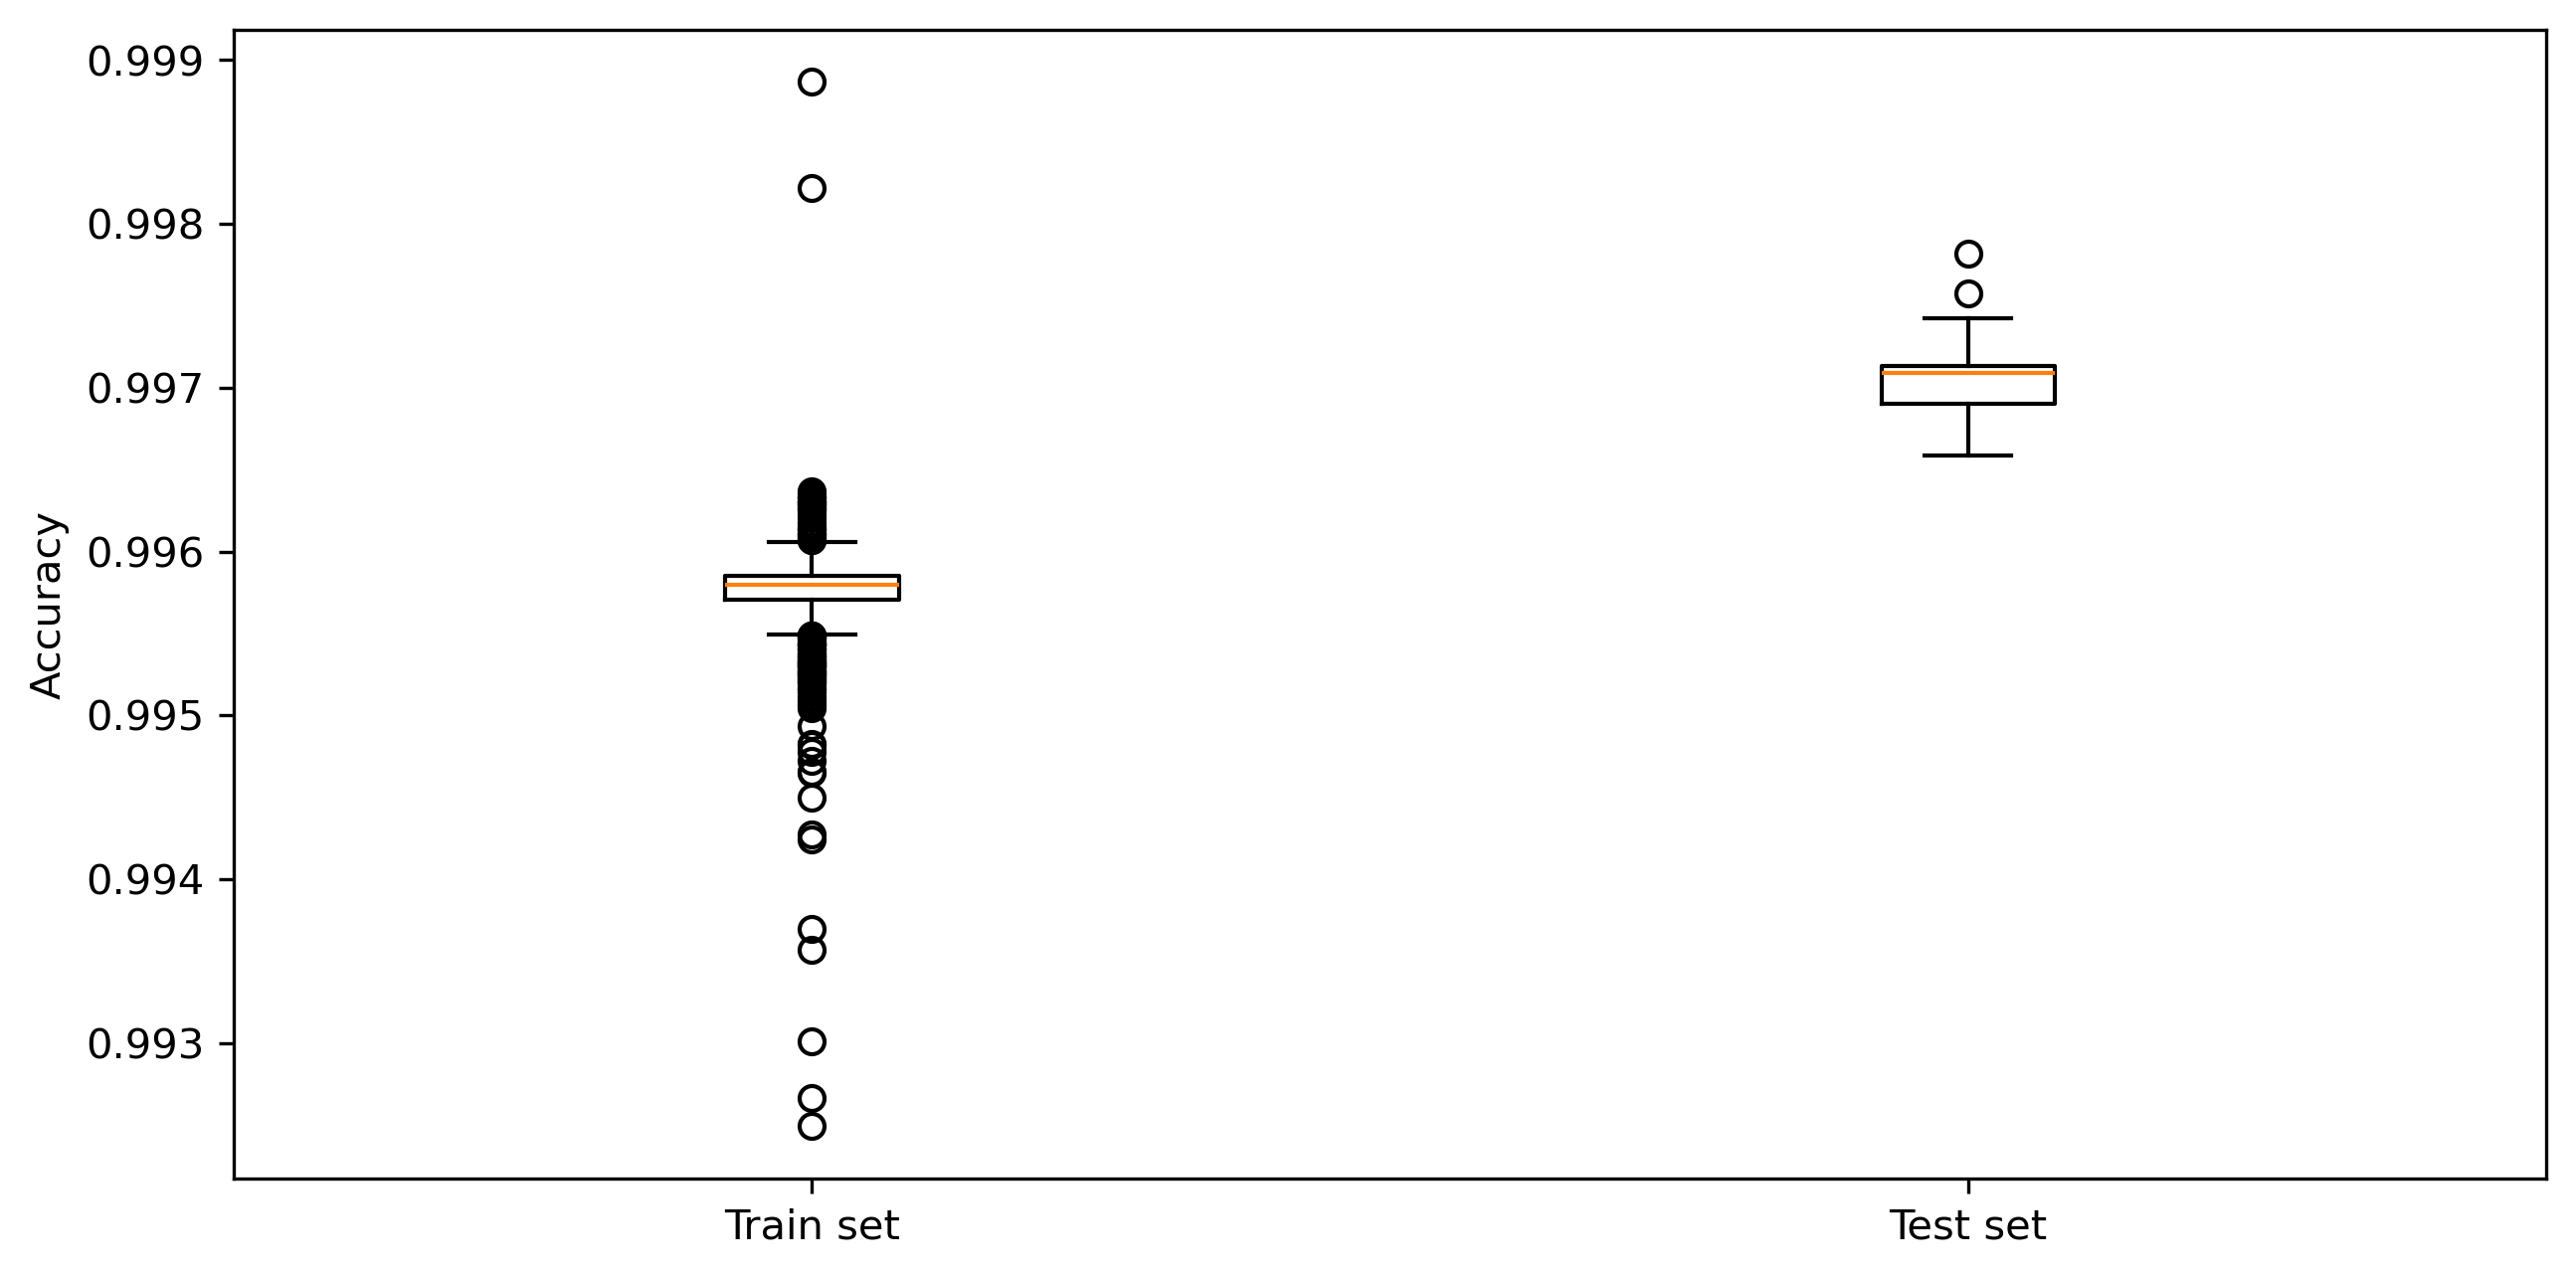
\includegraphics[width=0.8\textwidth]{figs/accuracy_boxplot.png}
    \caption{Boxplot of binary accuracies for the train and test sets.}
    \label{fig:accuracy_dist_box}

\end{figure}

\begin{figure}[H]
    \centering
    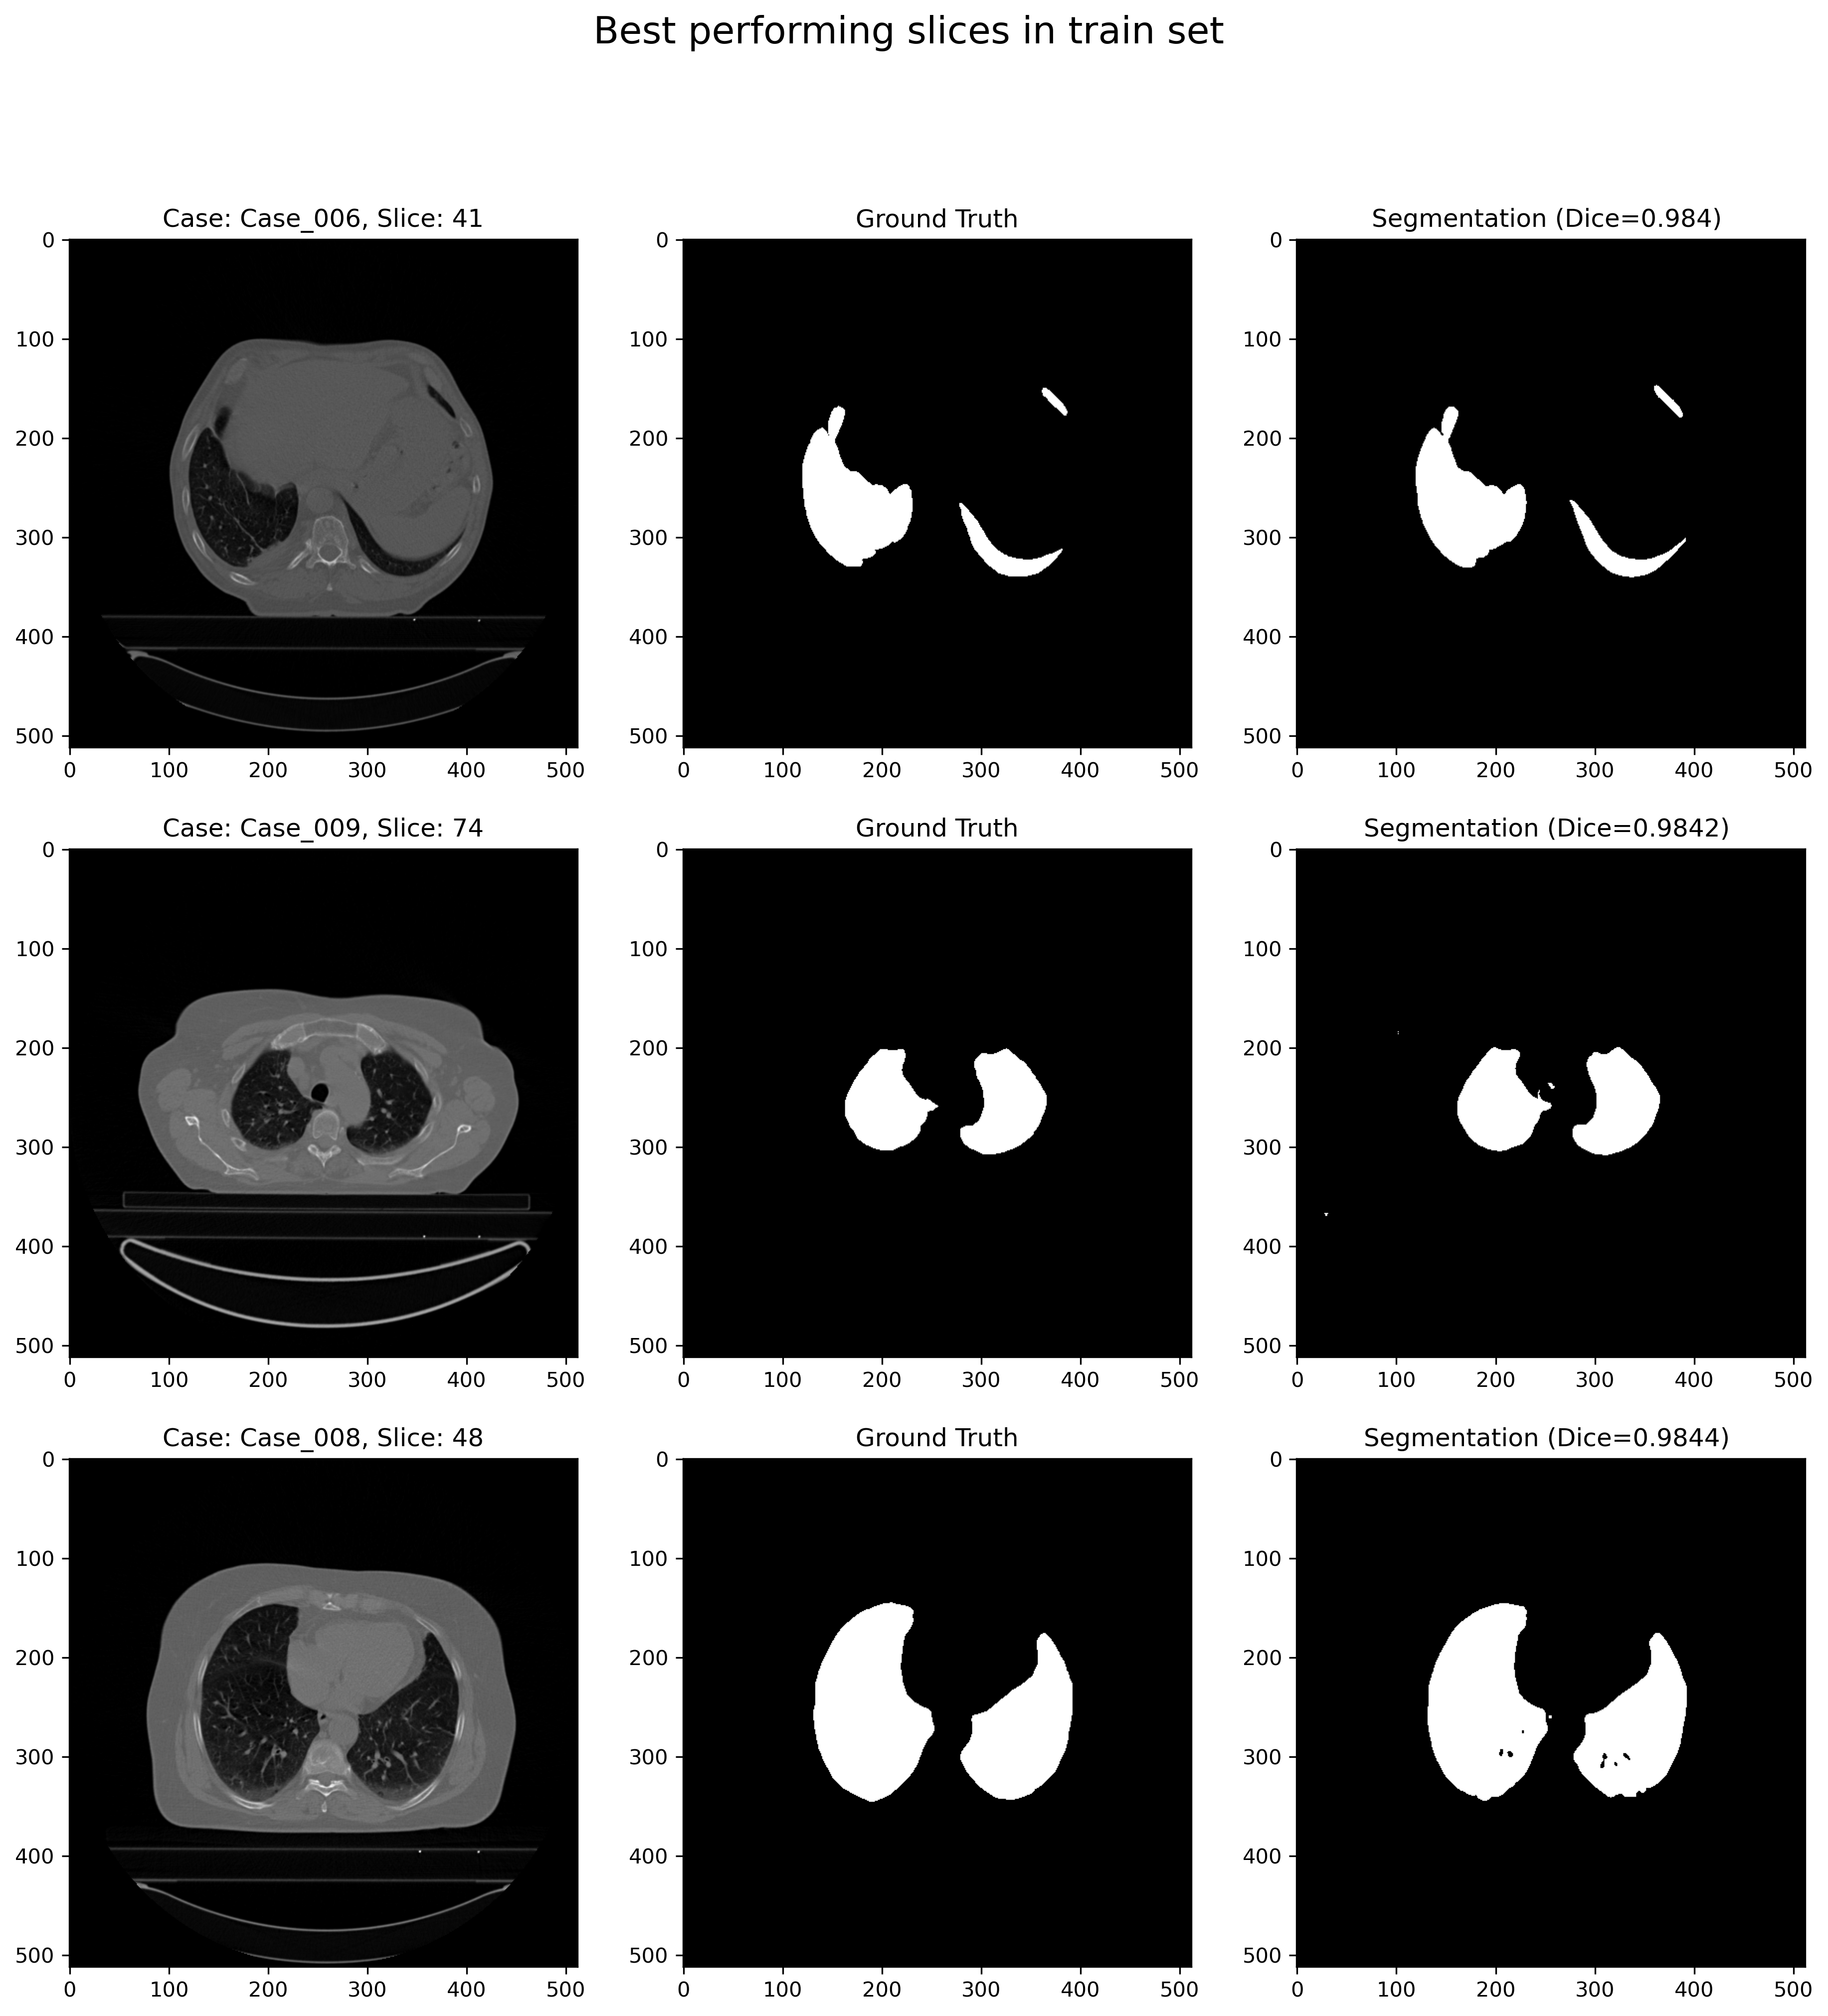
\includegraphics[width=0.5\textwidth]{figs/Best performing slices in train set.png}
    \caption{Comparison of the predicted masks with the ground truth masks for the train set. Cases from the train set with the top 3 dice scores as shown.}
    \label{fig:best_train_mask_comparison}
\end{figure}

\begin{figure}[H]
    \centering
    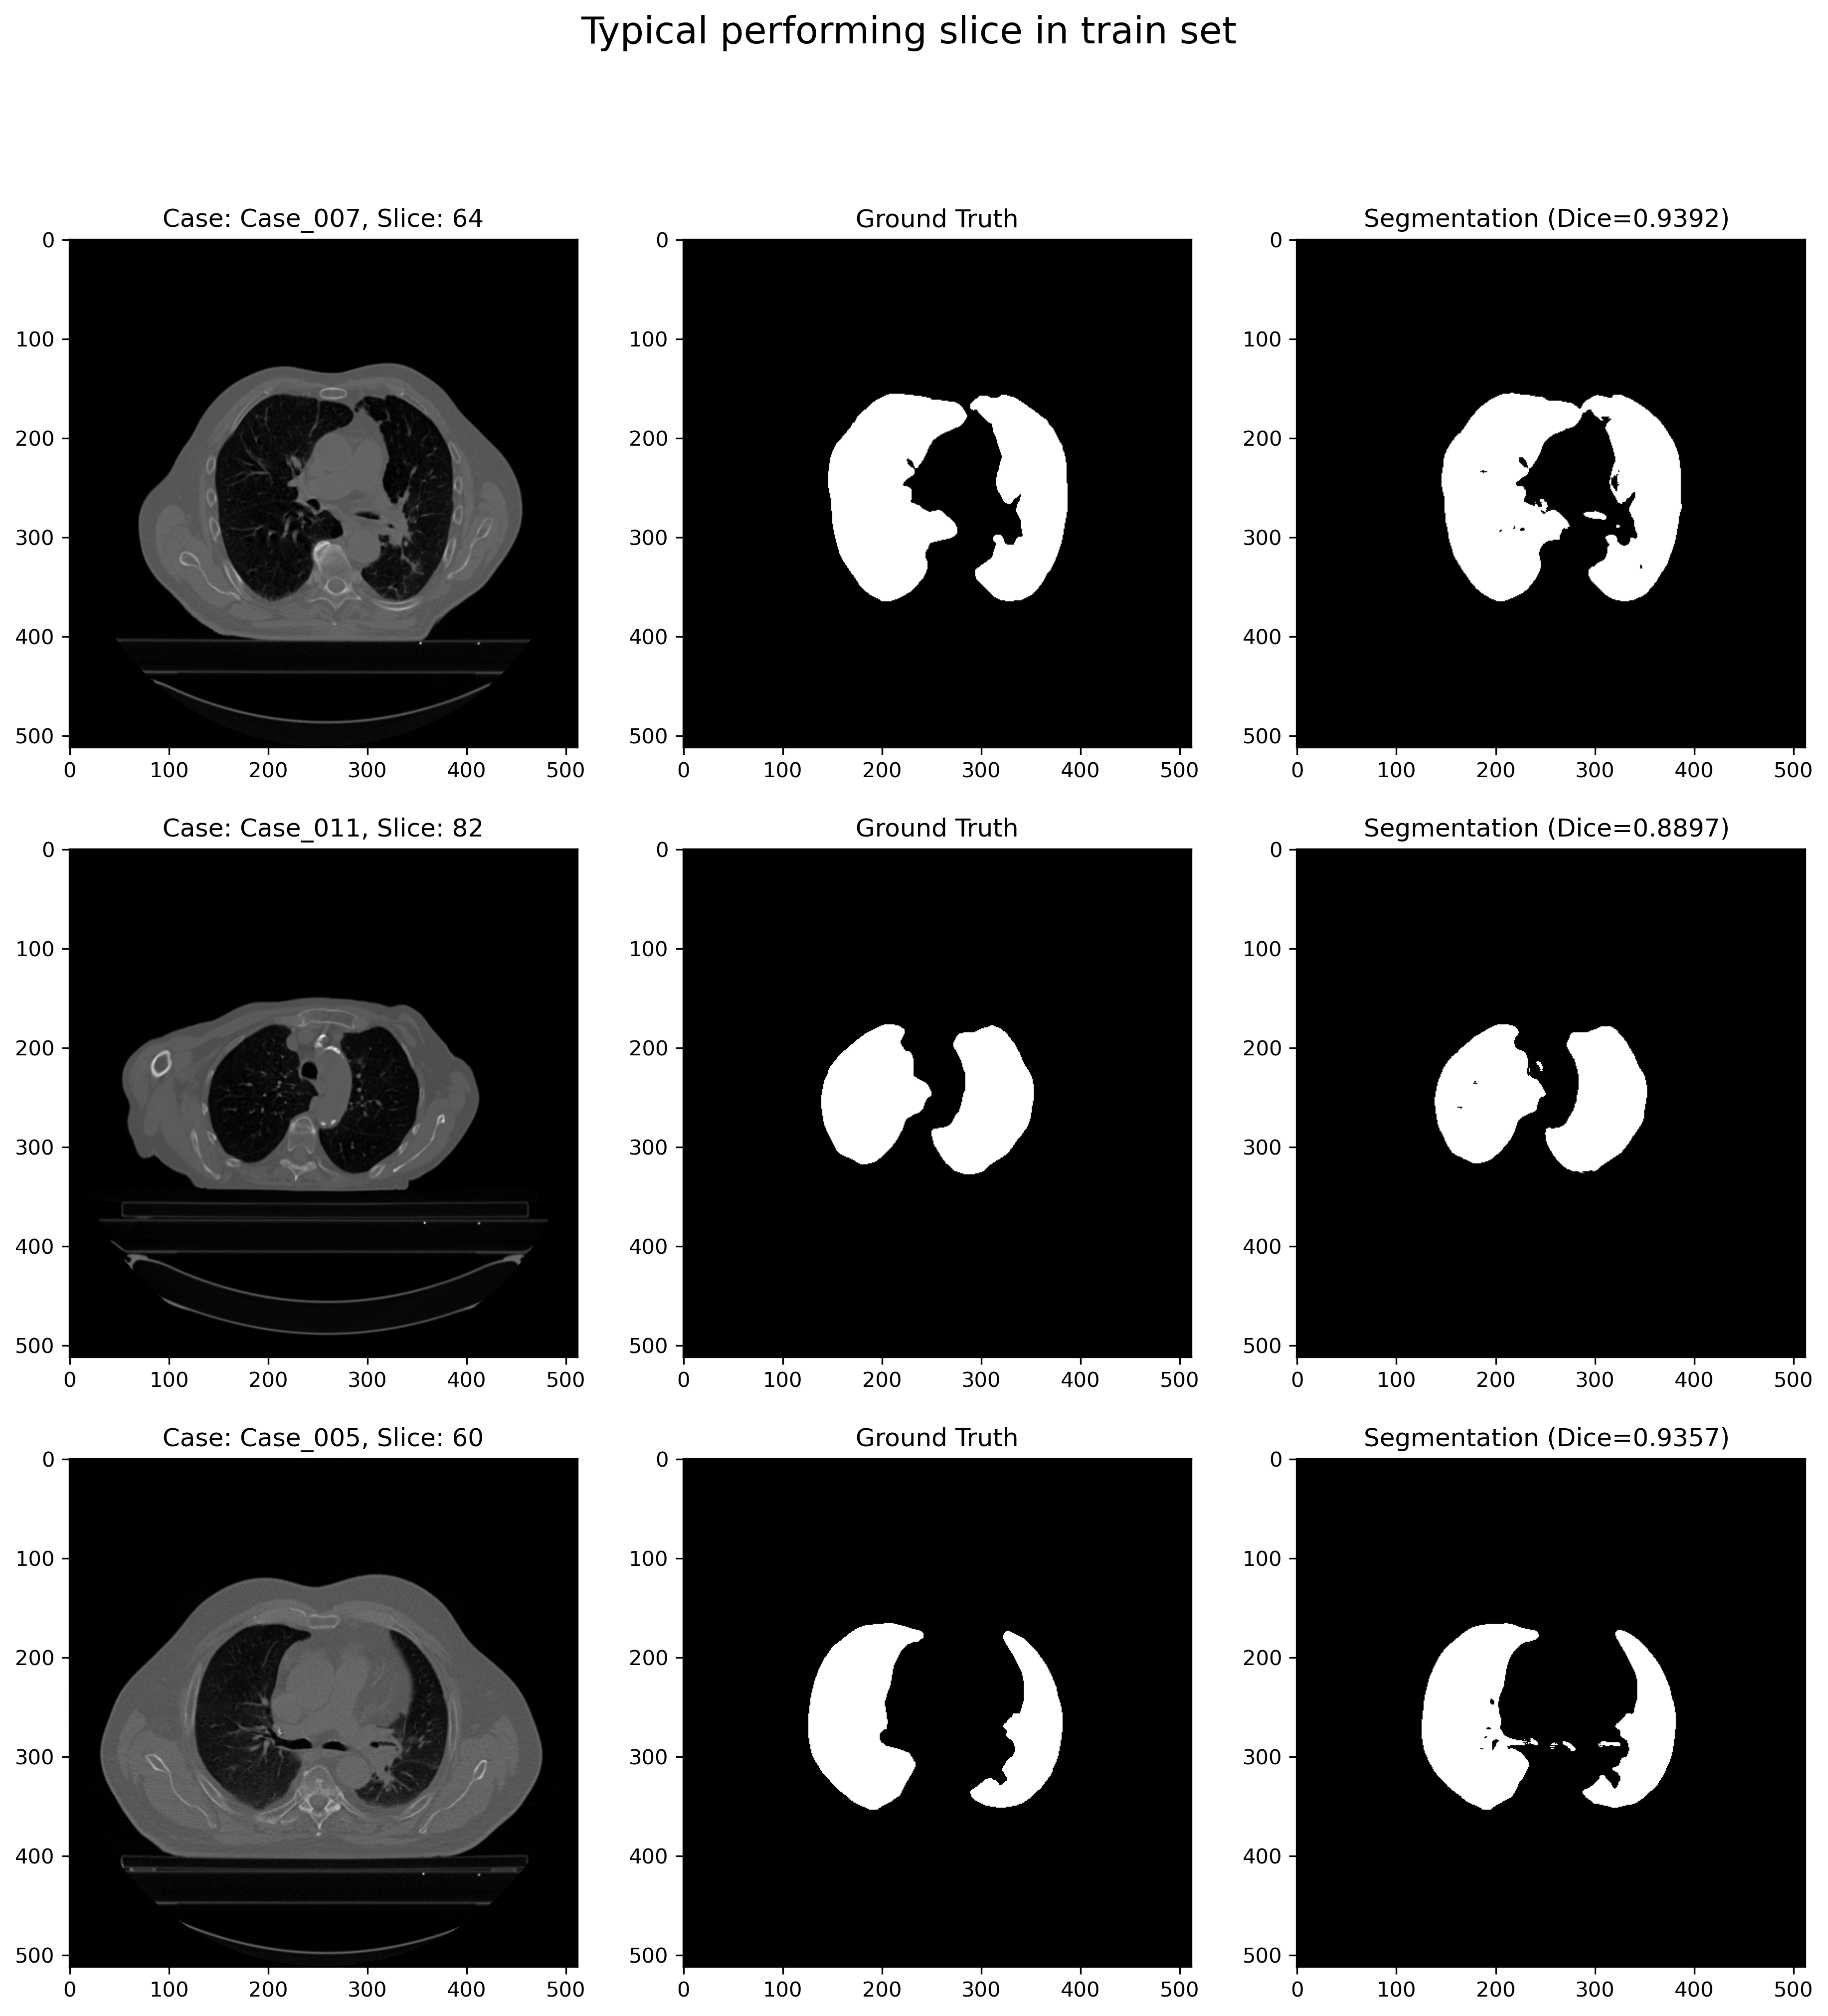
\includegraphics[width=0.5\textwidth]{figs/Typical performing slice in train set.png}
    \caption{Comparison of the predicted masks with the ground truth masks for the train set. 3 random cases from the train set with dice scores in the IQR are shown.}
    \label{fig:typical_train_mask_comparison}
\end{figure}

\begin{figure}[H]
    \centering
    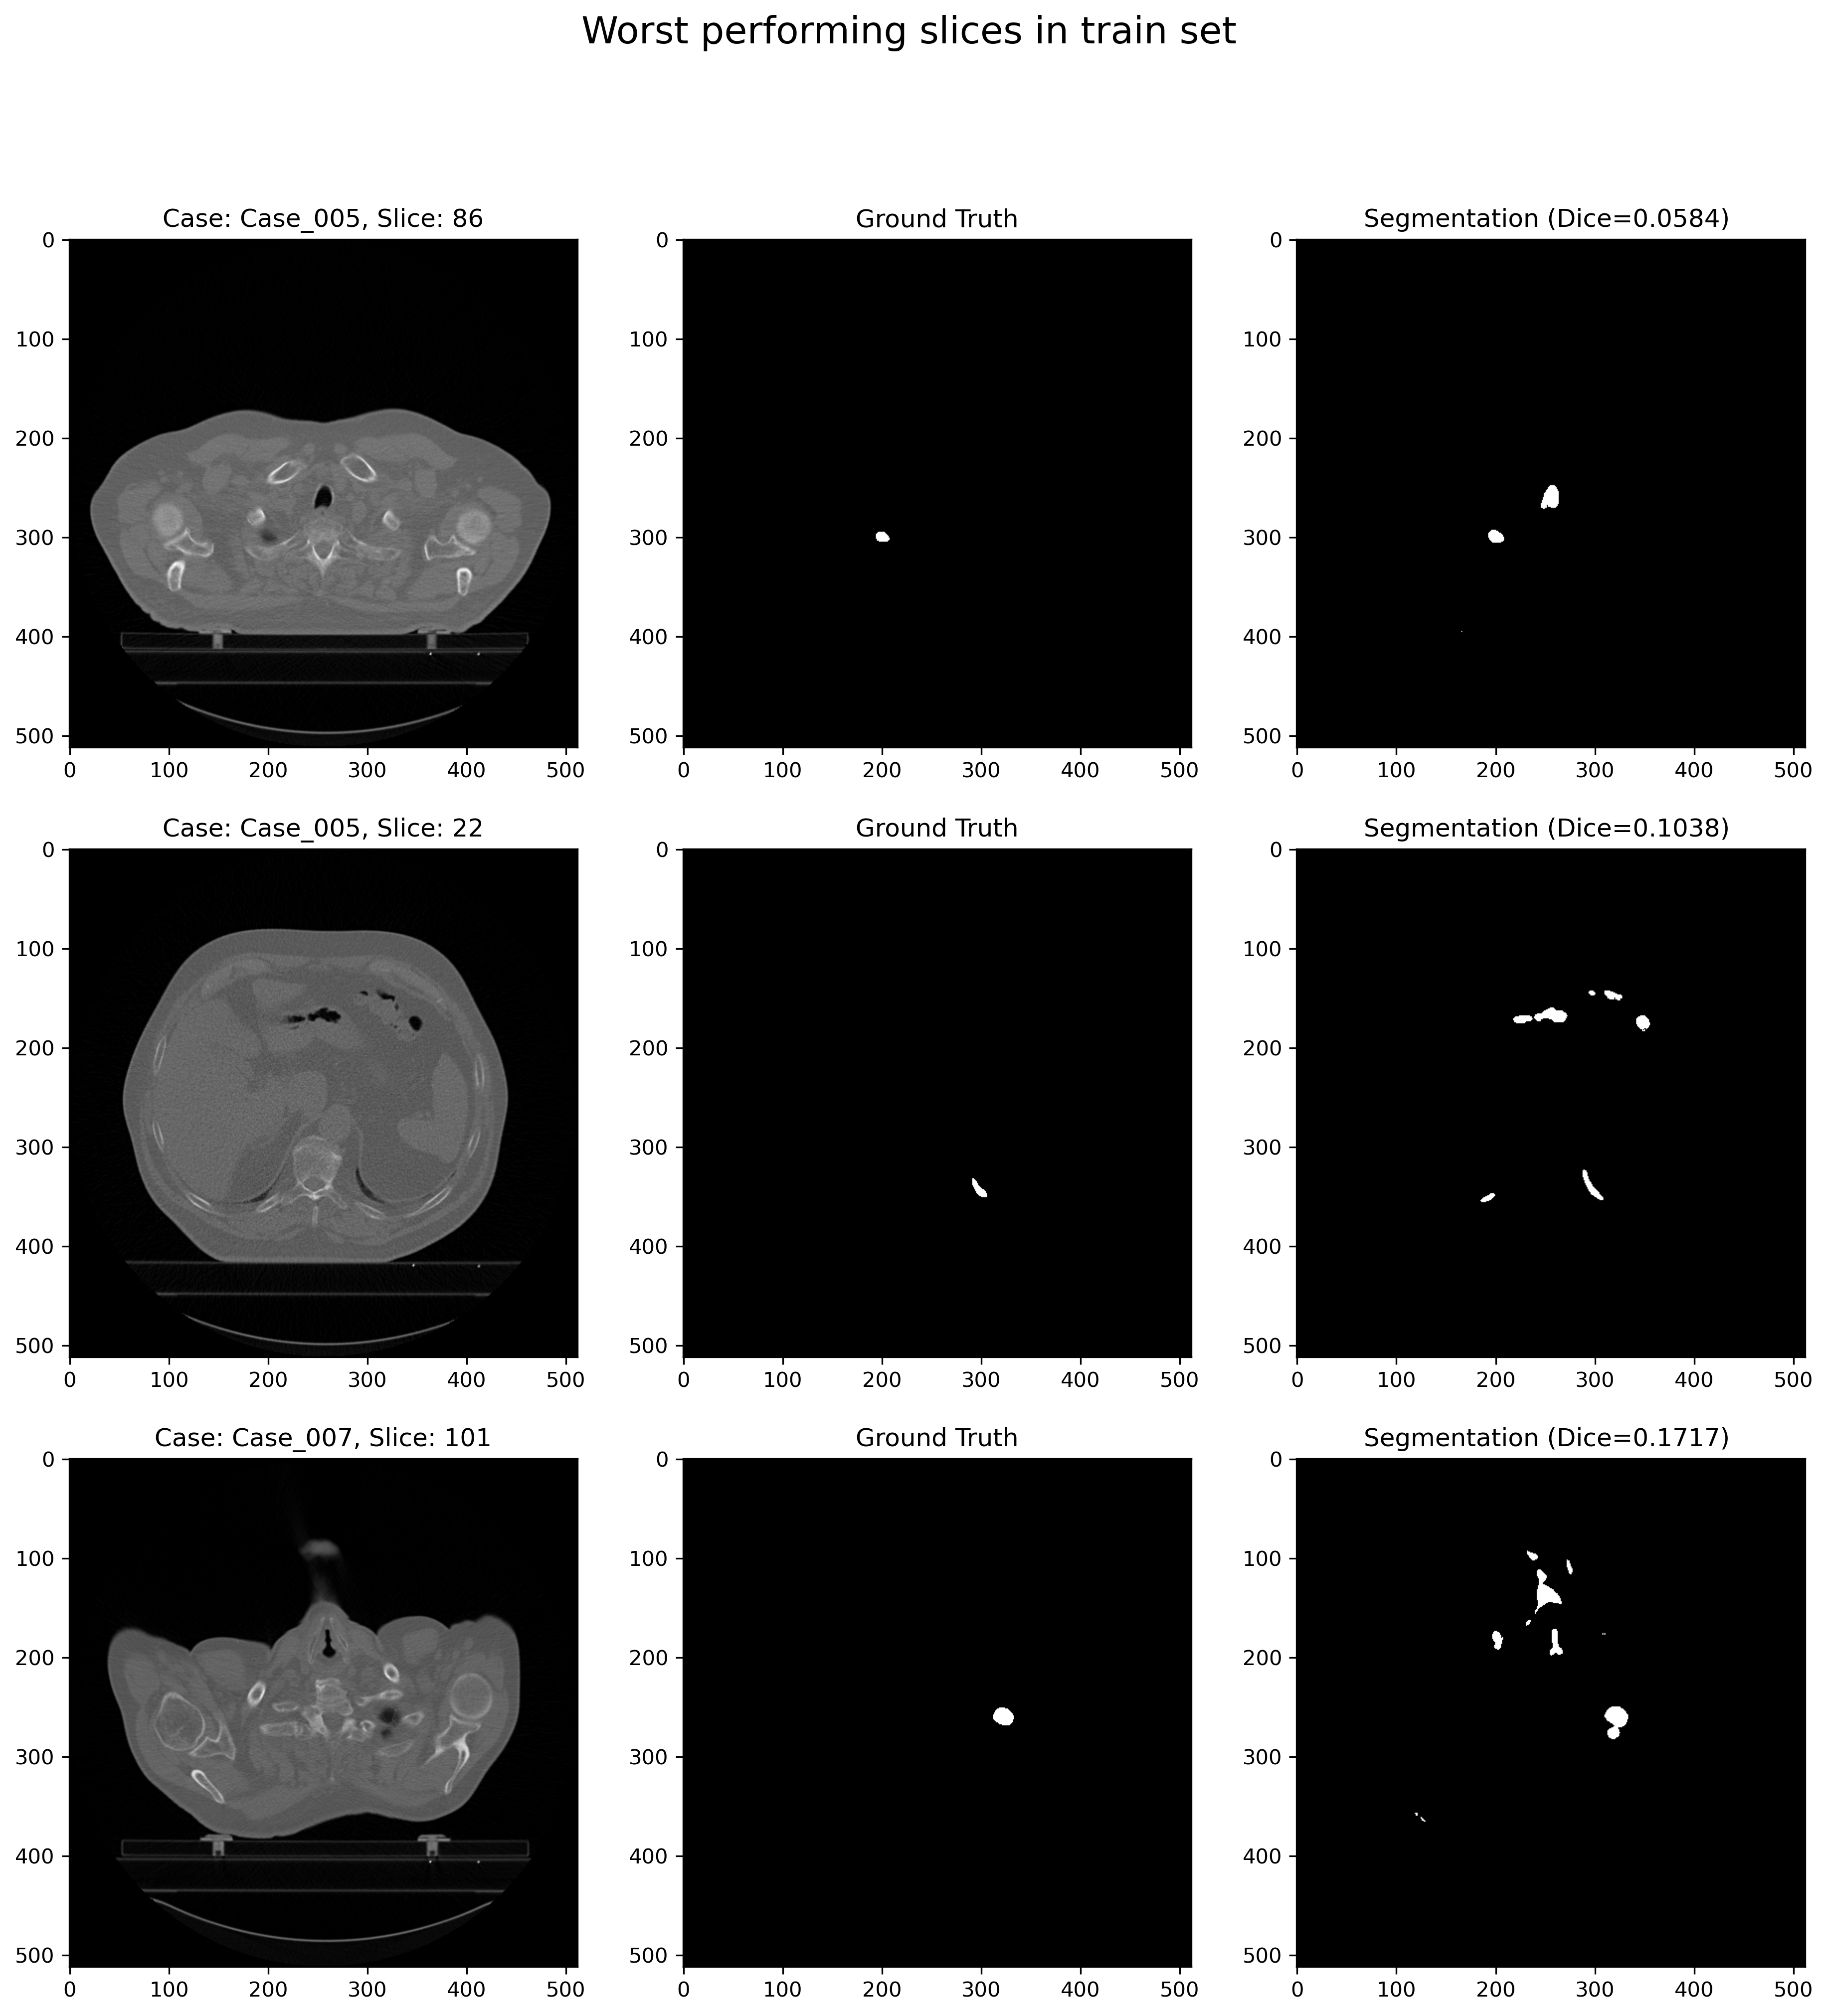
\includegraphics[width=0.5\textwidth]{figs/Worst performing slices in train set.png}
    \caption{Comparison of the predicted masks with the ground truth masks for the train set. Cases from the train set with the worst 3 dice scores as shown.}
    \label{fig:worst_train_mask_comparison}
\end{figure}

\begin{figure}[H]
    \centering
    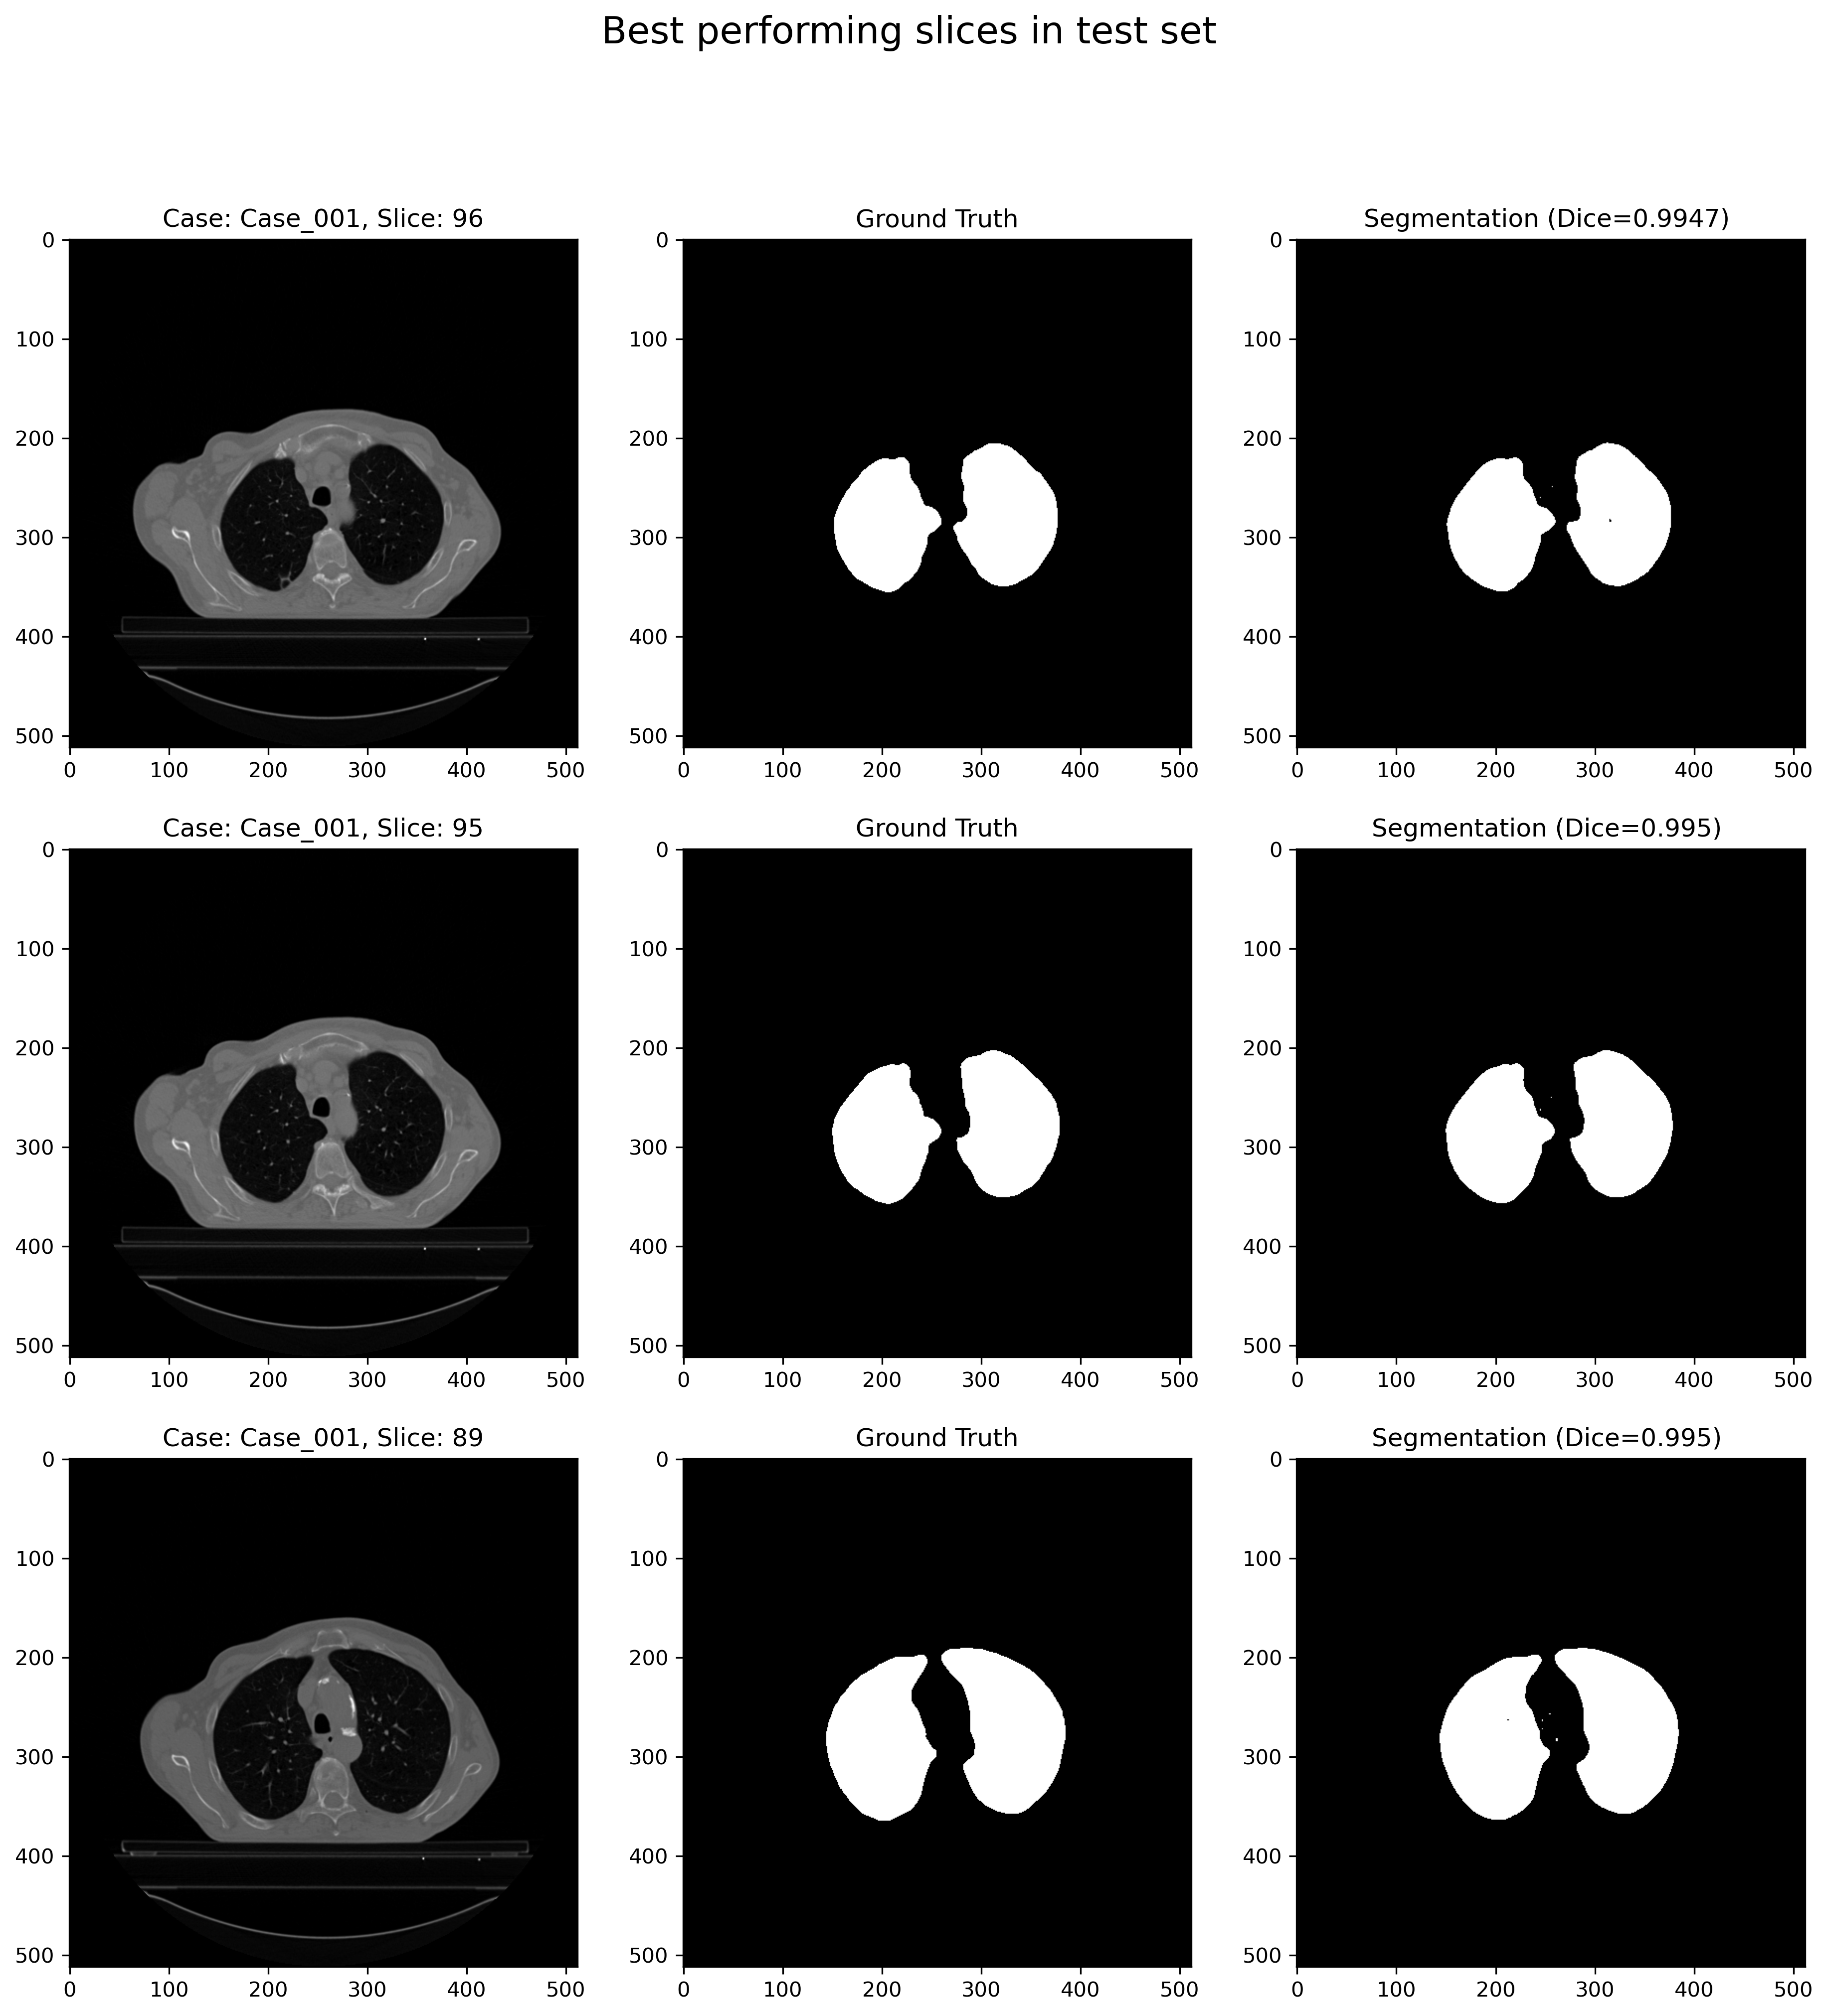
\includegraphics[width=0.5\textwidth]{figs/Best performing slices in test set.png}
    \caption{Comparison of the predicted masks with the ground truth masks for the test set. Cases from the test set with the best 3 dice scores as shown.}
    \label{fig:best_test_mask_comparison}
\end{figure}

\begin{figure}[H]
    \centering
    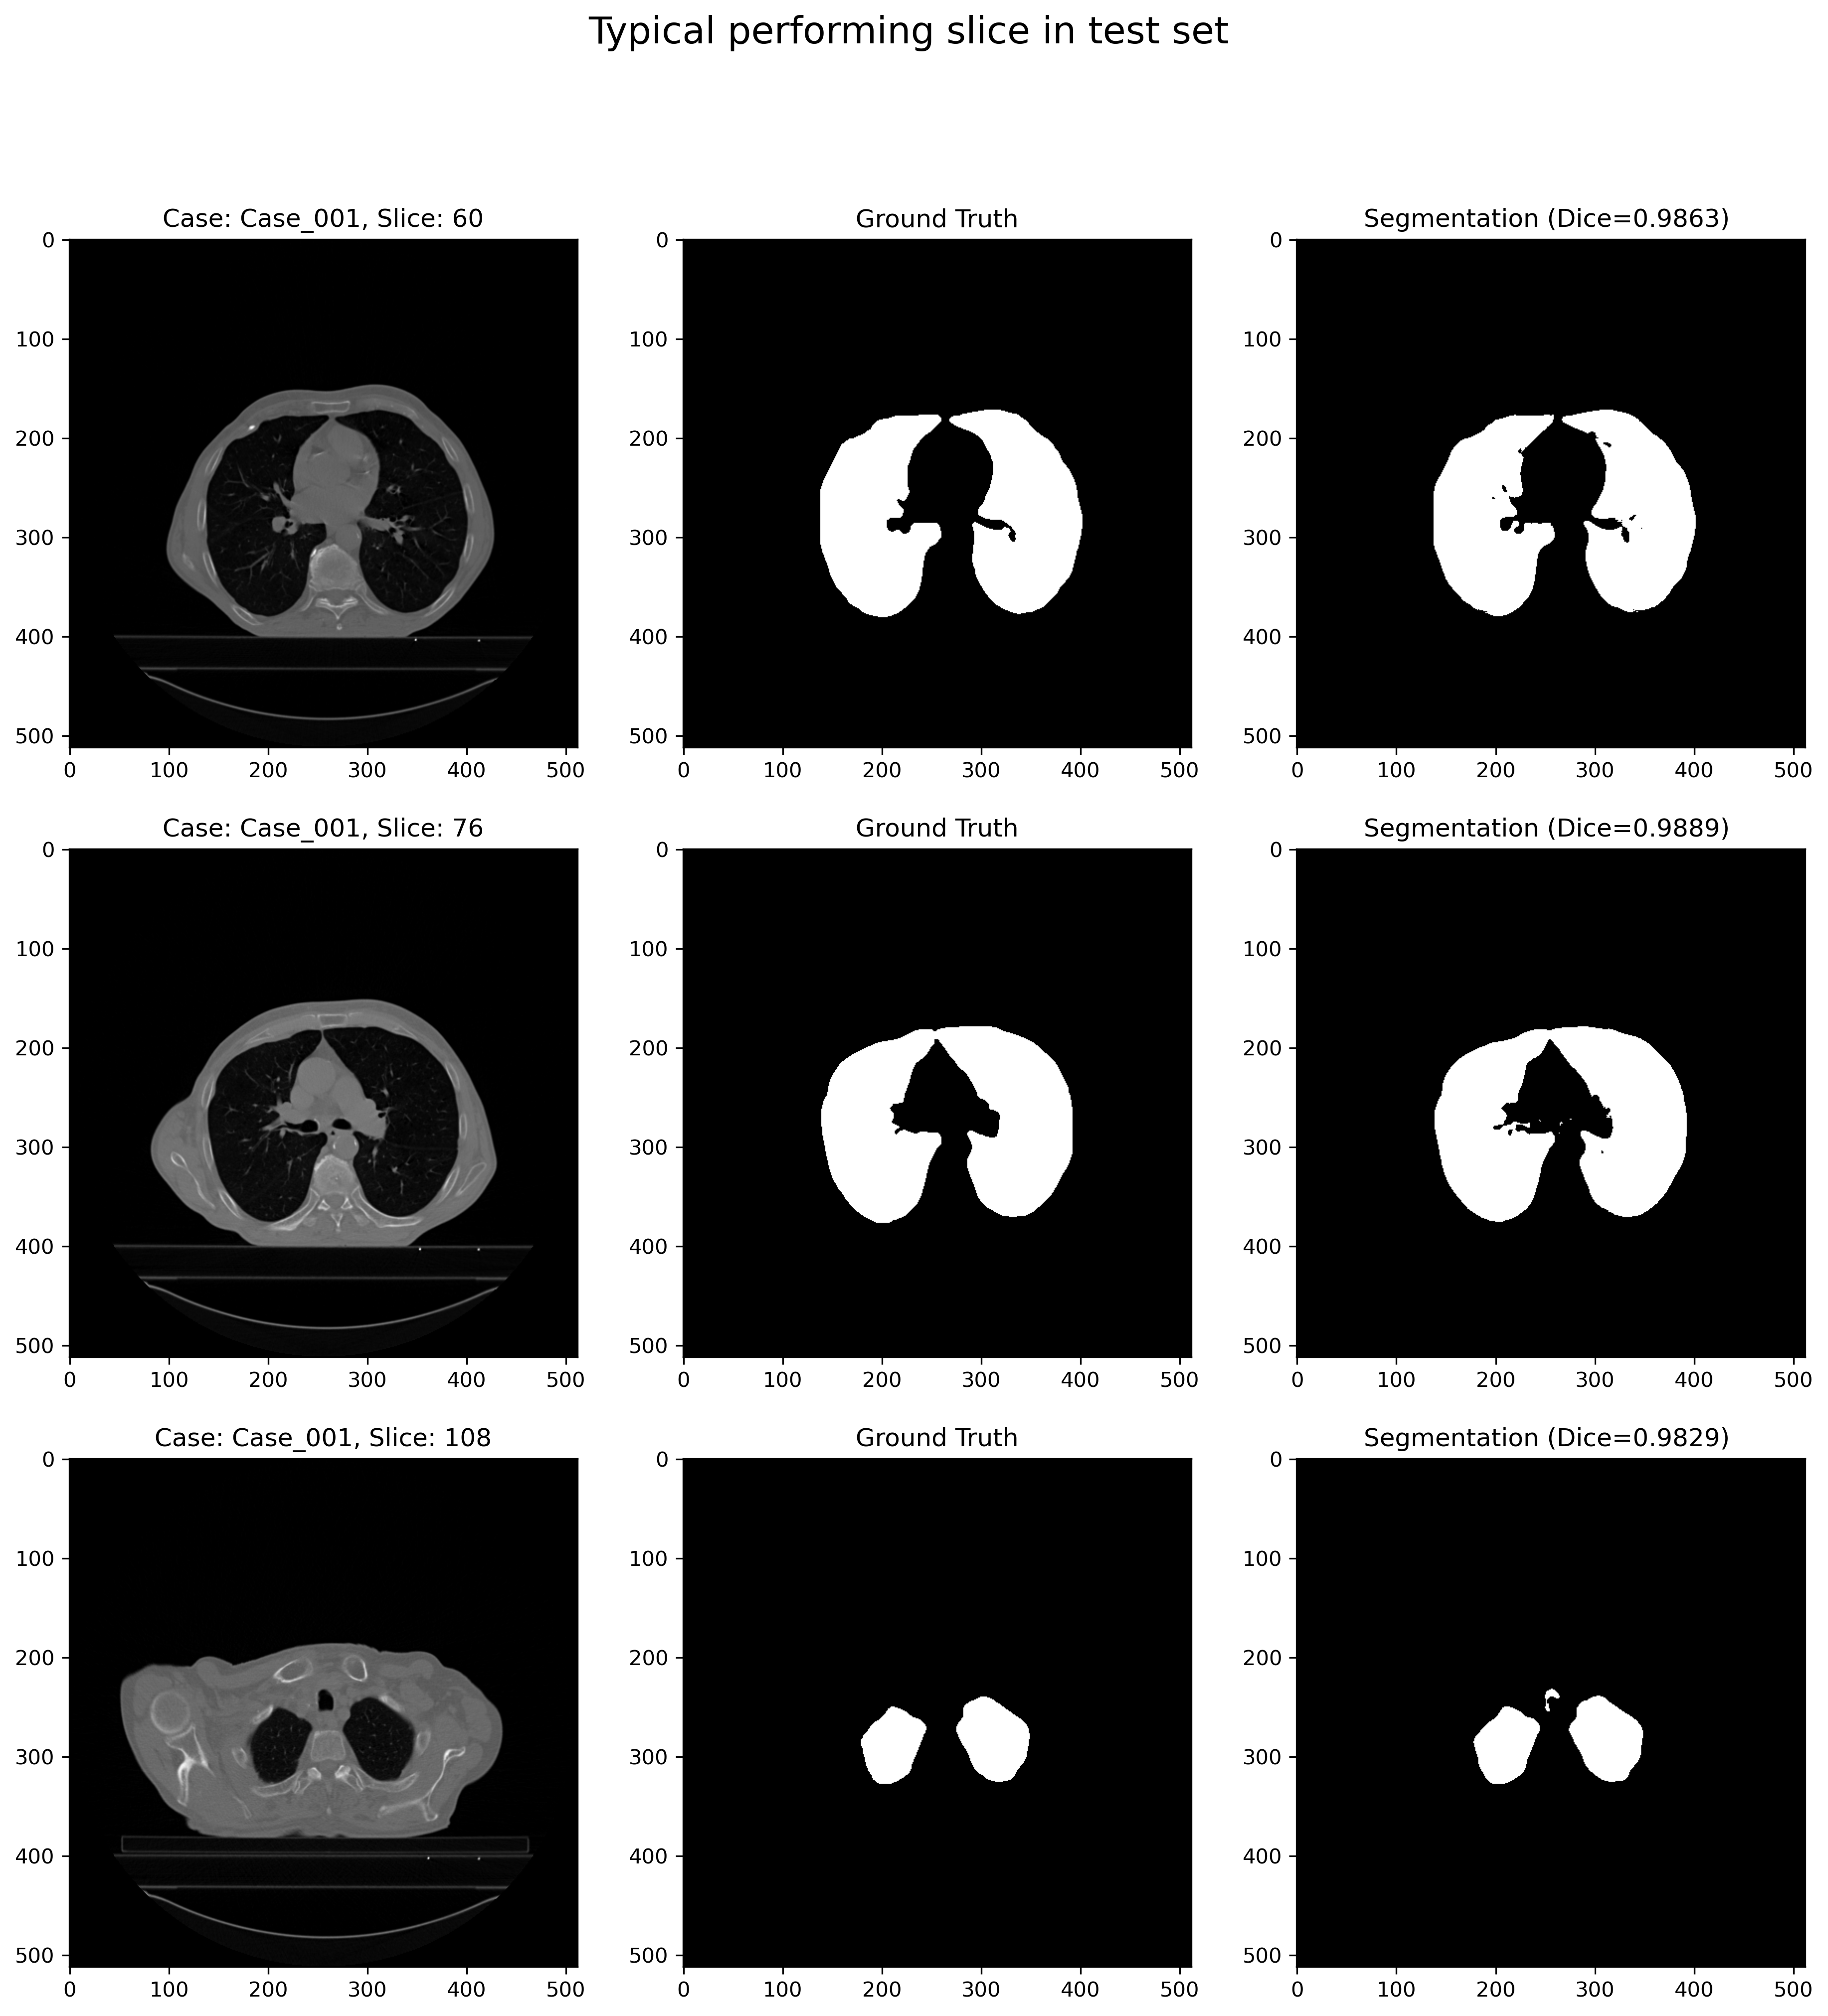
\includegraphics[width=0.5\textwidth]{figs/Typical performing slice in test set.png}
    \caption{Comparison of the predicted masks with the ground truth masks for the test set. 3 random cases from the test set with dice scores in the IQR are shown.}
    \label{fig:typical_test_mask_comparison}
\end{figure}

\begin{figure}[H]
    \centering
    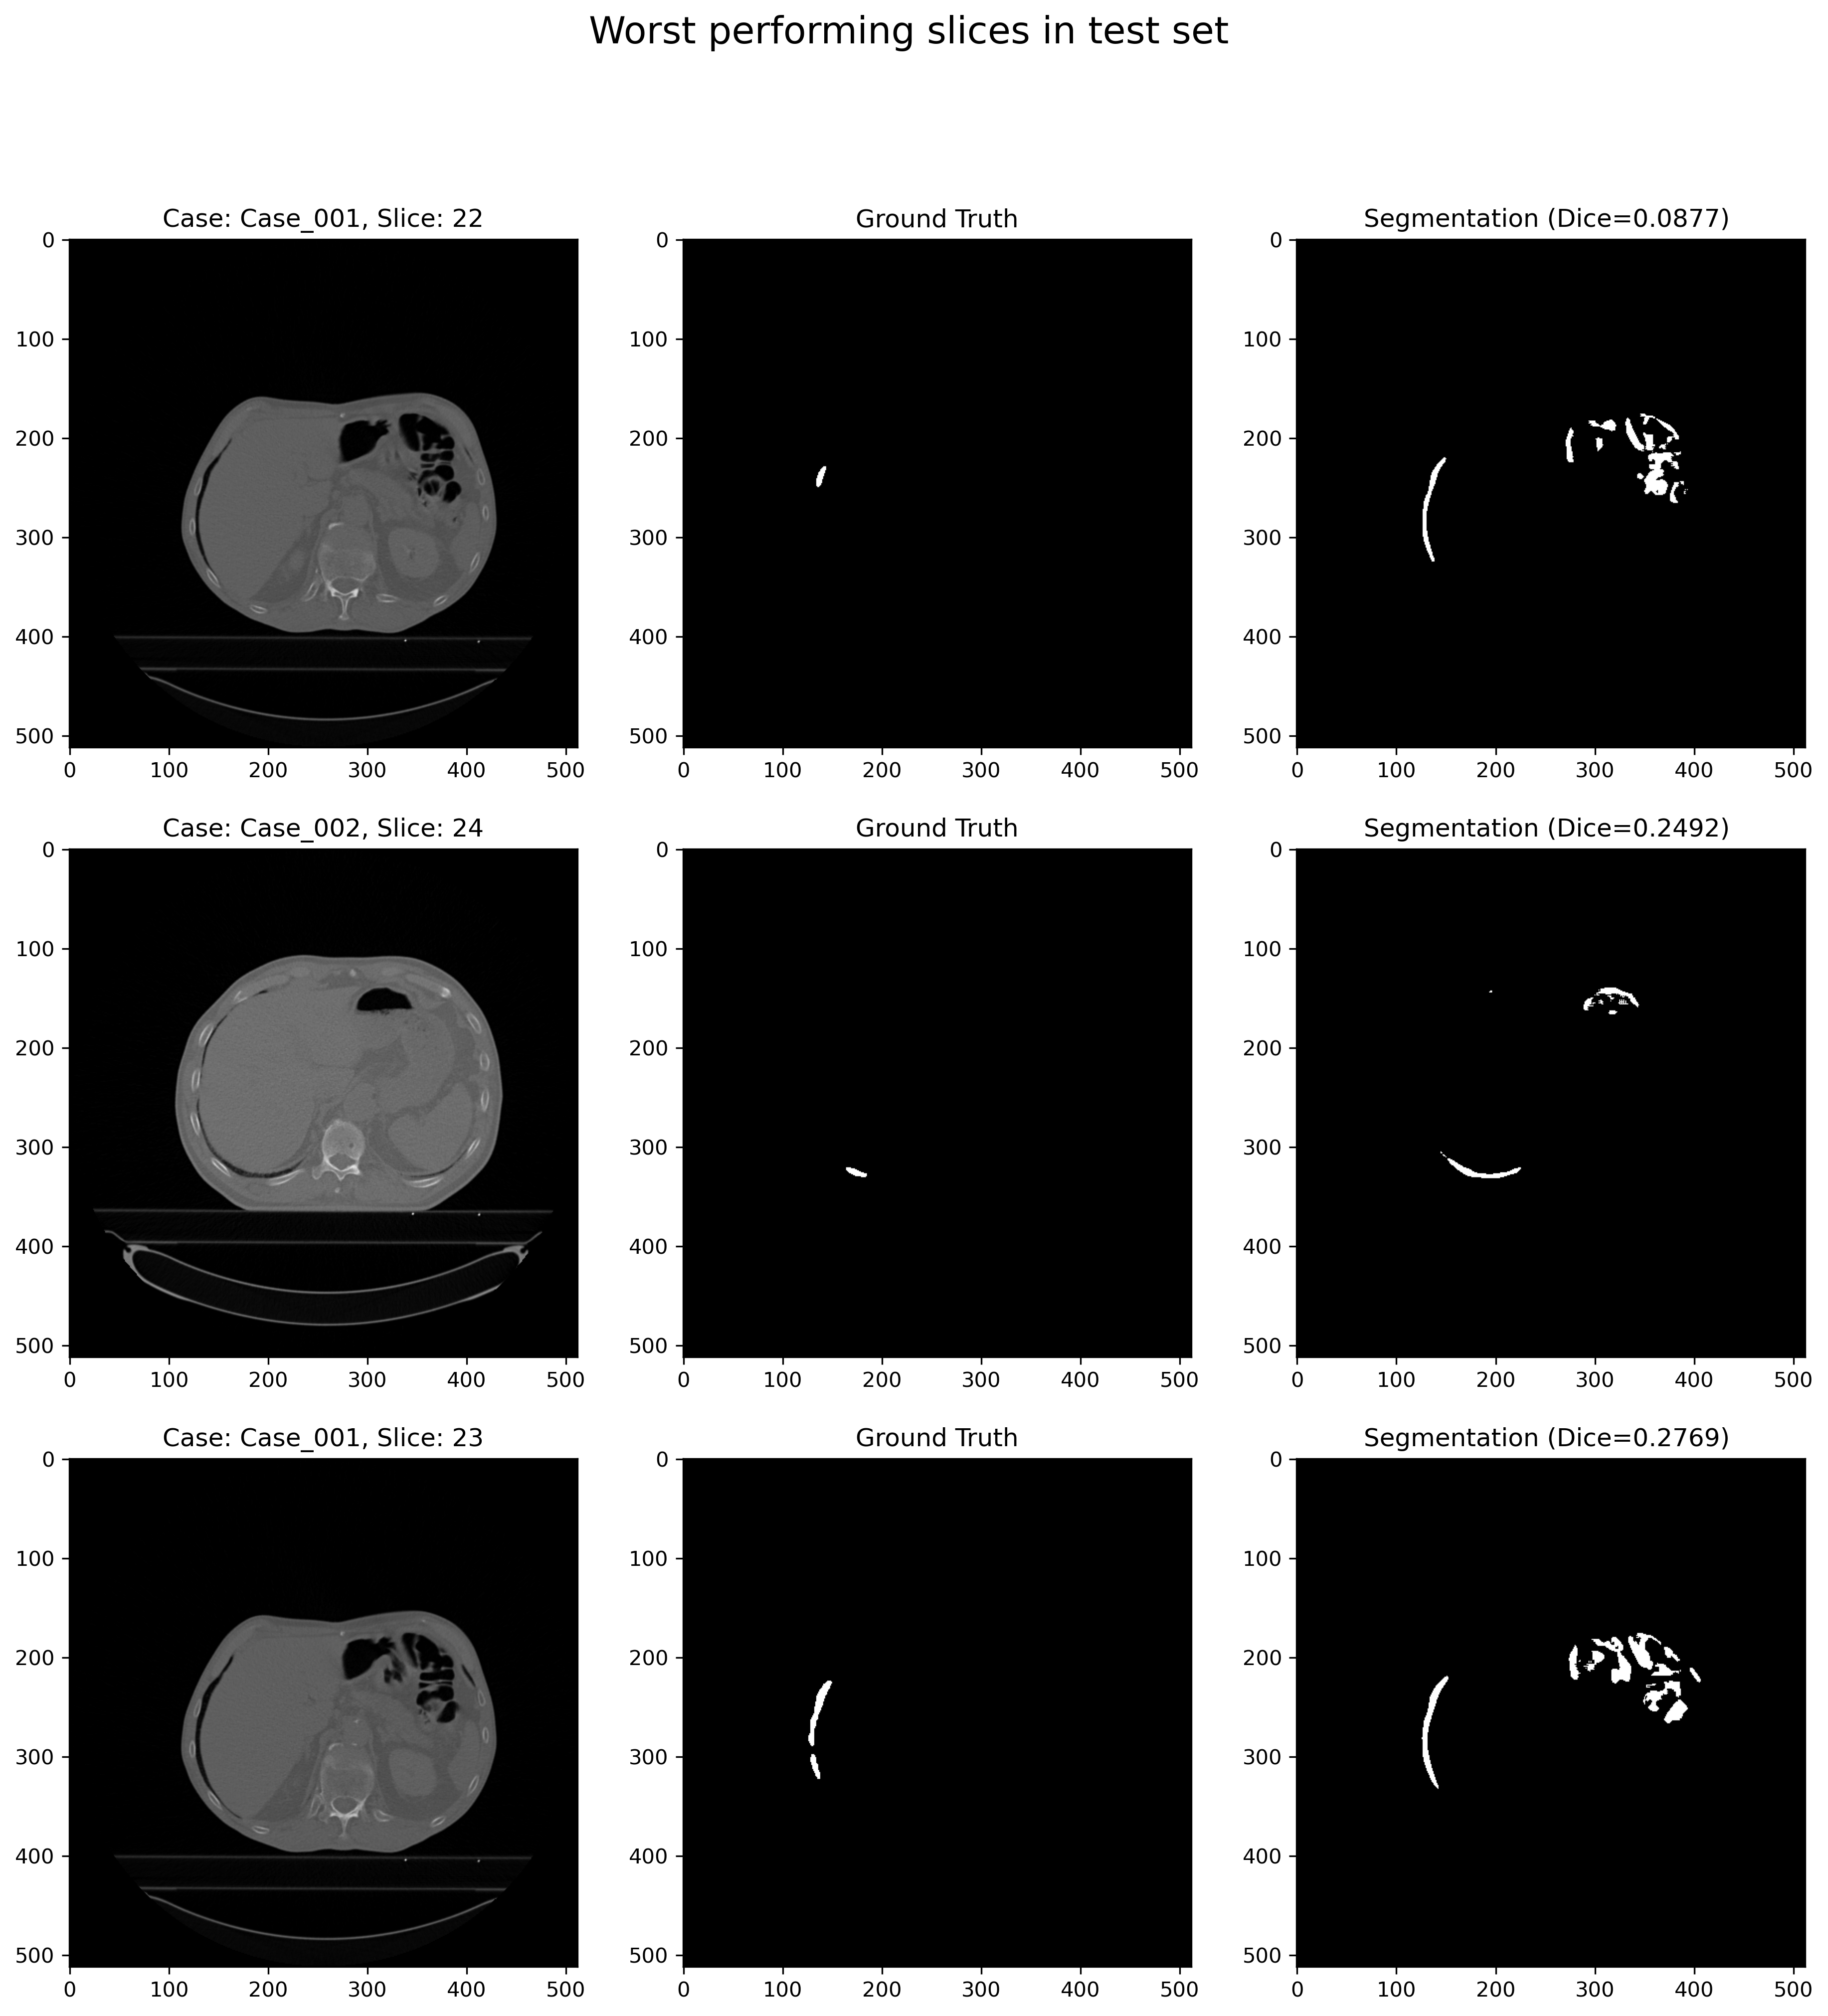
\includegraphics[width=0.5\textwidth]{figs/Worst performing slices in test set.png}
    \caption{Comparison of the predicted masks with the ground truth masks for the test set. Cases from the test set with the worst 3 dice scores as shown.}
    \label{fig:worst_test_mask_comparison}
\end{figure}

\subsection{Discussion and Future Work}
Clear trends can be established from looking at the best and worst cases from the final model on both the train and test sets.
Firstly, the model performs well on cases where the lungs are prominent and well-defined, as seen in the best cases. Conversely, the model struggles with cases where the lungs are less distinct, as seen in the worst cases. This is likely due to data imbalance, there are by definition going to be fewer edge slices which contain small amounts of lung tissue compared to the central slices which contain the majority of the lung tissue. As such, the model has less data to learn how to identify the lungs in the superior and inferior most axial slices which contain the lungs. Further, it is likely that the most variation in the lung shape and position occurs precisely in these slices which there are few samples of. Future work could involve data resampling techniques to address this imbalance, such as oversampling the edge slices or using data augmentation techniques to artificially generate more edge slices. Further, exploring architectures in which information between slices can be shared, such as 3D convolutions or recurrent neural networks, could be beneficial in better segmenting the lungs in the edge slices. This is because these architectures can leverage the clearer visibility of lungs in central slices to improve segmentation accuracy in edge slices, where lung tissue is minimal and less defined. 
One may wonder how it is possible the train loss shown in fig \ref{fig:loss_plot} seems to plateau at 0.25, indicating average dice scores of 0.75, while the average dice scores presented in table \ref{tab:dice_scores} are around 0.95? The answer lies in the fact during training many slices contained no lung tissue. The masks for such cases were all zeros and the dice loss was 1 regardless of the model prediction. This was not a problem for model optimisation as all the gradients would simply propate through the binary cross entropy loss term. However, it does heavily inflate the train loss as many batches would contain these background slices which would always have a dice loss of 1 regardless of the models agreement. This is why the train loss is so high compared to the test loss. Future work would also address this shortcoming of the training script. One final topic that could be addressed is contrasting these results with those of running the same model however windowing the intensities to the lung window. This would effectively mask out all the tissue that is not lung tissue and would allow the model to focus on the lung tissue alone. This could improve the model's performance on the edge slices as they would have greater contrast with the surround tissue.


\section{Conclusion}
In summary, this report presents a thorough exploration of the subset of the LCTSC dataset given as part of this coursework and trains a 2D UNet model for lung segmentation. The model achieves good performance with an average dice score of 0.949 and an average binary accuracy of 0.997 on the test set. The model struggles with cases where the lungs are less distinct, likely due to data imbalance. Future work could involve data resampling techniques to address this imbalance, such as oversampling the edge slices or using data augmentation techniques to artificially generate more edge slices. Further, exploring architectures in which information between slices can be shared, such as 3D convolutions or recurrent neural networks, could be beneficial in better segmenting the lungs in the edge slices.


\section{Appendix}
\subsection{CoPilot and ChatGPT usage}
CoPilot was used heavily when writing the code in \texttt{src/figs.ipynb}. It was 
also used to create the docstrings shown in this repo. It was also used to format and generate the latex for the figures and tables in this report.


\end{document}